\documentclass[11pt]{scrartcl}
\usepackage[T1]{fontenc}
\usepackage[utf8]{inputenc}
\usepackage{graphicx}
\usepackage{amsmath,amsfonts,amssymb, amsthm}
\usepackage{bm}
\usepackage{graphicx}
\usepackage{color}
\usepackage{rotating}
\usepackage{cite}
\usepackage{textcomp}
\usepackage{lmodern}
\usepackage{color}
\usepackage{chngcntr}
% makes Fig number in the form Fig. <Section-Nr>.number with number being reset after every section (i.e. new blog entry)
\counterwithin{figure}{section}
\counterwithin{equation}{section}
\usepackage{hyperref}
\usepackage{makeidx}
\usepackage{float}
\usepackage{subcaption}
\makeindex

%\usepackage{pstricks}

\usepackage{tikz}
\usetikzlibrary{arrows,%
                petri,%
                topaths}%
\usepackage{tkz-berge}


\newcommand{\abf}{\mathbf{a}}
\newcommand{\bbf}{\mathbf{b}}
\newcommand{\cbf}{\mathbf{c}}
\newcommand{\dbf}{\mathbf{d}}
\newcommand{\ebf}{\mathbf{e}}
\newcommand{\fbf}{\mathbf{f}}
\newcommand{\gbf}{\mathbf{g}}
\newcommand{\hbf}{\mathbf{h}}
\newcommand{\ibf}{\mathbf{i}}
\newcommand{\jbf}{\mathbf{j}}
\newcommand{\kbf}{\mathbf{k}}
\newcommand{\lbf}{\mathbf{l}}
\newcommand{\mbf}{\mathbf{m}}
\newcommand{\nbf}{\mathbf{n}}
\newcommand{\obf}{\mathbf{o}}
\newcommand{\pbf}{\mathbf{p}}
\newcommand{\qbf}{\mathbf{q}}
\newcommand{\rbf}{\mathbf{r}}
\newcommand{\sbf}{\mathbf{s}}
\newcommand{\tbf}{\mathbf{t}}
\newcommand{\ubf}{\mathbf{u}}
\newcommand{\vbf}{\mathbf{v}}
\newcommand{\wbf}{\mathbf{w}}
\newcommand{\xbf}{\mathbf{x}}
\newcommand{\ybf}{\mathbf{y}}
\newcommand{\zbf}{\mathbf{z}}



\newcommand{\Abf}{\mathbf{A}}
\newcommand{\Bbf}{\mathbf{B}}
\newcommand{\Cbf}{\mathbf{C}}
\newcommand{\Dbf}{\mathbf{D}}
\newcommand{\Ebf}{\mathbf{E}}
\newcommand{\Fbf}{\mathbf{F}}
\newcommand{\Gbf}{\mathbf{G}}
\newcommand{\Hbf}{\mathbf{H}}
\newcommand{\Ibf}{\mathbf{I}}
\newcommand{\Kbf}{\mathbf{K}}
\newcommand{\Lbf}{\mathbf{L}}
\newcommand{\Mbf}{\mathbf{M}}
\newcommand{\Nbf}{\mathbf{N}}
\newcommand{\Obf}{\mathbf{O}}
\newcommand{\Pbf}{\mathbf{P}}
\newcommand{\Rbf}{\mathbf{R}}
\newcommand{\Sbf}{\mathbf{S}}
\newcommand{\Tbf}{\mathbf{T}}
\newcommand{\Ubf}{\mathbf{U}}
\newcommand{\Vbf}{\mathbf{V}}
\newcommand{\Wbf}{\mathbf{W}}
\newcommand{\Xbf}{\mathbf{X}}
\newcommand{\Ybf}{\mathbf{Y}}
\newcommand{\Zbf}{\mathbf{Z}}

\newcommand{\zerobf}{\mathbf{0}}
\newcommand{\onebf}{\mathbf{1}}
\newcommand{\Sigmabf}{\mathbf{\Sigma}}

\newcommand{\Ac}{\mathcal{A}}
\newcommand{\Dc}{\mathcal{D}}
\newcommand{\Ec}{\mathcal{E}}
\newcommand{\Gc}{\mathcal{G}}
\newcommand{\Ic}{\mathcal{I}}
\newcommand{\Nc}{\mathcal{N}}
\newcommand{\CNc}{\mathcal{CN}}
\newcommand{\Oc}{\mathcal{O}}
\newcommand{\Qc}{\mathcal{Q}}
\newcommand{\Cc}{\mathcal{C}}
\newcommand{\Sc}{\mathcal{S}}
\newcommand{\Vc}{\mathcal{V}}
\newcommand{\Zc}{\mathcal{Z}}

\newcommand{\mC}{\mathbb{C}}
\newcommand{\mF}{\mathbb{F}}
\newcommand{\mZ}{\mathbb{Z}}

\newcommand{\erf}{\mathrm{erf}}
\newcommand{\Exp}{\mathrm{E}}


\newcommand{\be}{\begin{equation}}
\newcommand{\ee}{\end{equation}}

\newcommand{\bee}{\begin{equation*}}
\newcommand{\eee}{\end{equation*}}



% a command to generate a new diary entry
% parameters: title, date, category
\newcommand{\DiaryEntry}[3]{
  \pagebreak
  %\vspace*{3mm}
  \section{#1, #2}\index{#3!#1 - #2}
  \vspace*{-3mm}
  \textit{#2 #3}

  \noindent\rule{8cm}{0.5pt}
  \vspace{3mm}
  \label{#2:entry}
}

\newtheorem{definition}{Definition}[section]
\newtheorem{theorem}{Theorem}[section]
\newtheorem{problem}{Problem}[section]


\begin{document}

\title{My Personal Journal}
\author{}
\date{}

\maketitle

\tableofcontents

\printindex

%\DiaryEntry{Least Squares}{2015-06-26}{Maths}


Derivation of the least-squares expression: Given the system matrix \(\mathbf{A}\) and the observation \(\mathbf{y}\), we seek the \(\mathbf{\hat{x}}\) so that the error \(\mathbf{r} = \mathbf{y} - \mathbf{A} \mathbf{x}\) is minimized.

%\pagebreak

\begin{figure}[htb!]
\centering
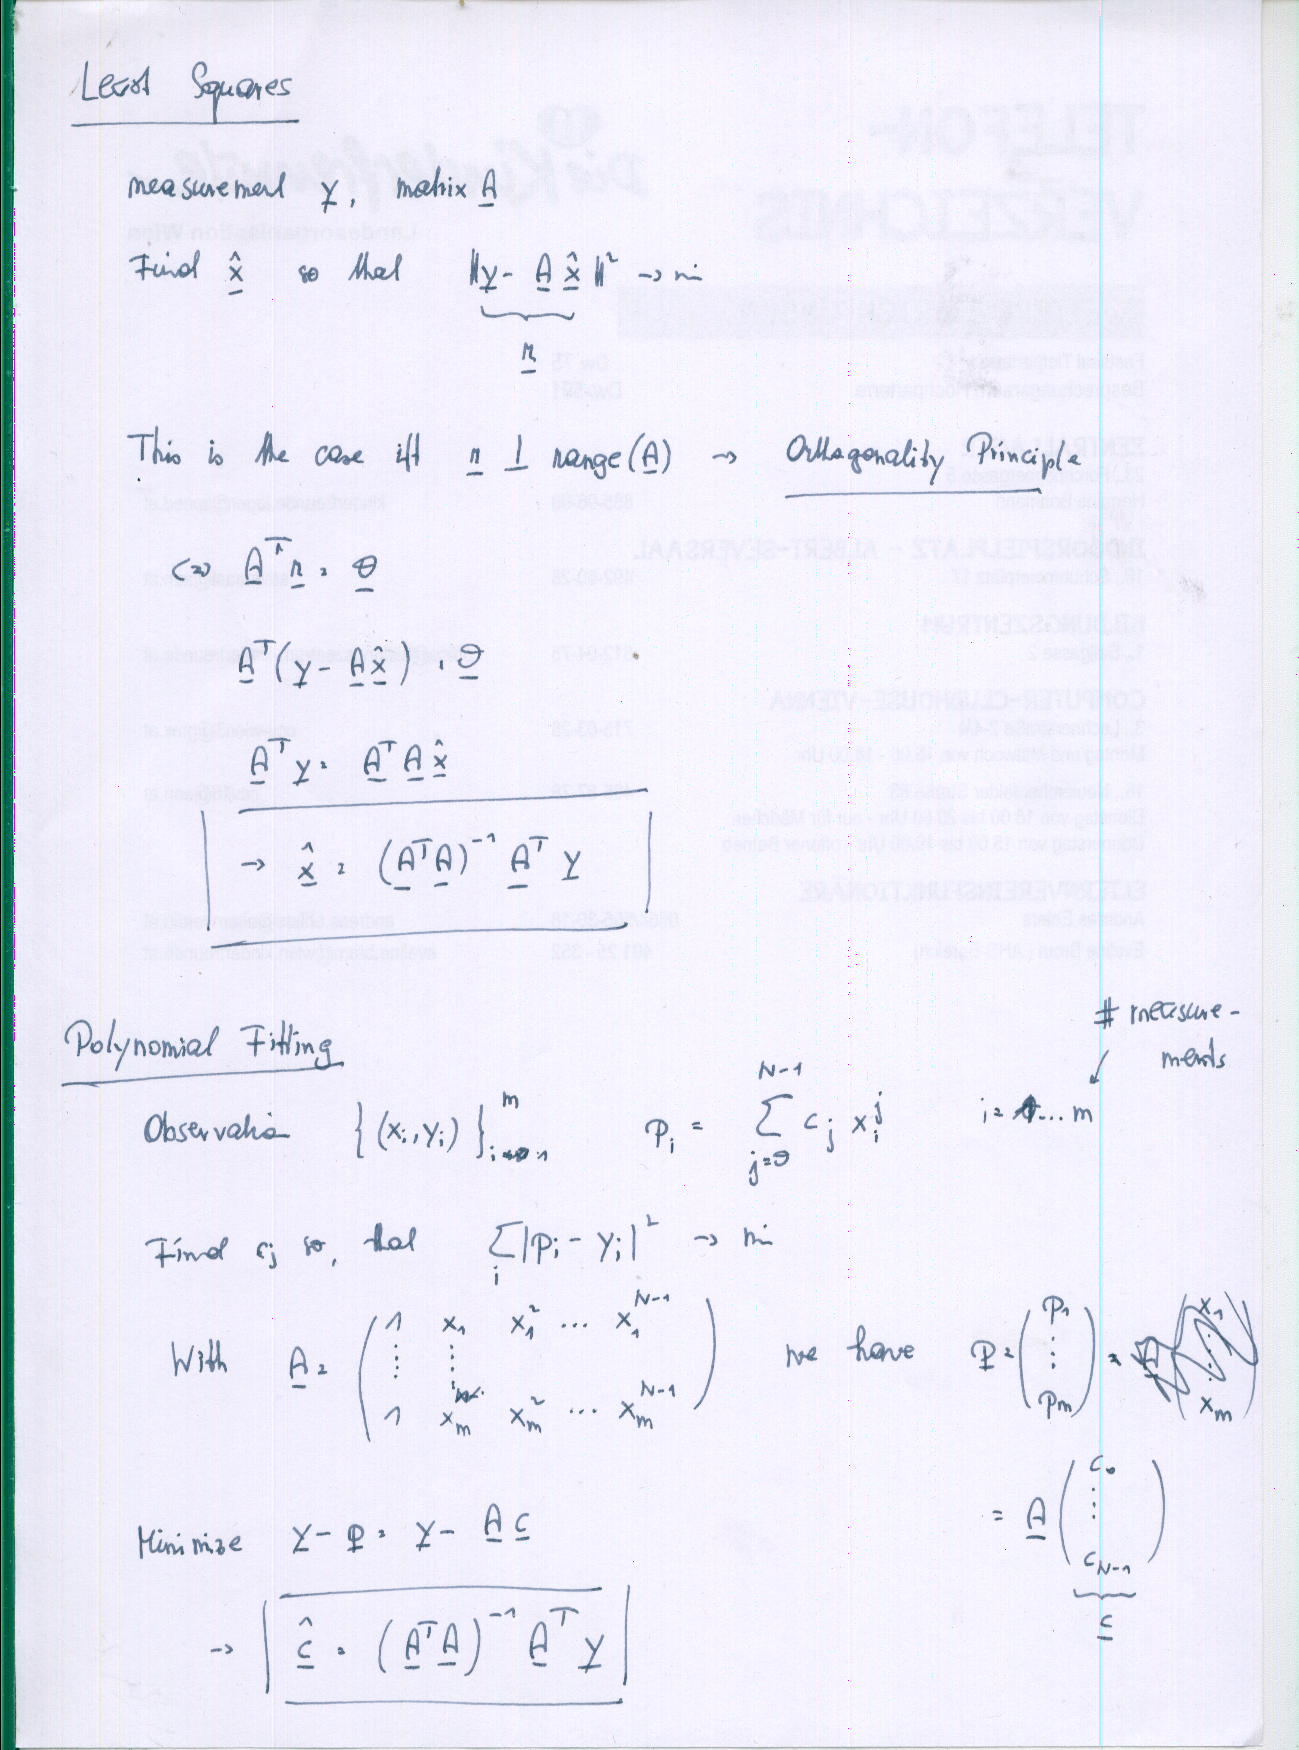
\includegraphics[scale=0.5]{images/least_squares.png}
\caption{Derivation}
\end{figure}

Seen another way, the result \(\mathbf{\hat{x}} = (\mathbf{A}^T \mathbf{A})^{-1} \mathbf{A}^T \mathbf{y}\) is the projection of \(\mathbf{y}\) onto the vector space defined by the columns of \(\mathbf{A}\).

\subsection{Least Squares Example (Julia)}

We consider \(\mathbb{R}^3\) and want to project onto the x-y plane; first we choose the matrix \(\mathbf{A} = [\mathbf{e_1} \mathbf{e_2}]\)

\begin{verbatim}
A=[1 0;0 1;0 0]
inv(A'*A)*A'

2x3 Array{Float64,2}:
1.0  0.0  0.0
0.0  1.0  0.0
\end{verbatim}

The least squares matrix considers only the first two components of any vector it is applied onto =\textgreater{} projection onto x-y plane.

Similarly, nothing (much) changes, if we choose different vectors \(\mathbf{u_1}, \mathbf{u_2}\) for \(\mathbf{A} = [\mathbf{u_1} \mathbf{u_2}]\), as long as they are part of the x-y plane:

\begin{verbatim}
A=[sqrt(2)/2 -sqrt(2)/2;sqrt(2)/2 sqrt(2)/2;0 0]

3x2 Array{Float64,2}:
0.707107  -0.707107
0.707107   0.707107
0.0        0.0     

inv(A'*A)*A'

2x3 Array{Float64,2}:
0.707107  0.707107  0.0
-0.707107  0.707107  0.0
\end{verbatim}

\subsection{Least Squares Polynomial Fitting Example (Julia)}

\subsubsection{No Noise}

We consider \(x_i={-2,-1.2,-0.4,0.4,1.2,2}\) and $y_i=x_i^3$. We least-squares fit three polynoms onto the point set \({x_i,y_i}\) with degree \(N=1\) (a straight line); \(N=3\) (a polynom of the same order as the ``model''), and \(N=6\); i.e. a polynomial with a higher order.

\begin{verbatim}
using Winston

N = 6
srand(1234)

x = linspace(-2,2,N)
y = x.^3

yobs = y

A1 = [x.^0 x.^1]
A3 = [x.^0 x.^1 x.^2 x.^3]
A5 = [x.^0 x.^1 x.^2 x.^3 x.^4 x.^5]


c_hat_1 = inv(A1'*A1)*A1'*yobs
c_hat_3 = inv(A3'*A3)*A3'*yobs
c_hat_5 = inv(A5'*A5)*A5'*yobs

plot(x,yobs,"-rx", x,A1*c_hat_1,"ob", x,A3*c_hat_3,"og", x,A5*c_hat_5,"oy")
savefig("ls_polyfit.pdf")
\end{verbatim}

The following plot shows the results for these different degrees. The observed data is shown in red with circles. The polynomial with $N=1$ (blue circles) gives a bad fit; both $N=3$ (green circles) and $N = 6$ (yellow pluses) yield a pefect match.

\begin{figure}[htb!]
\centering
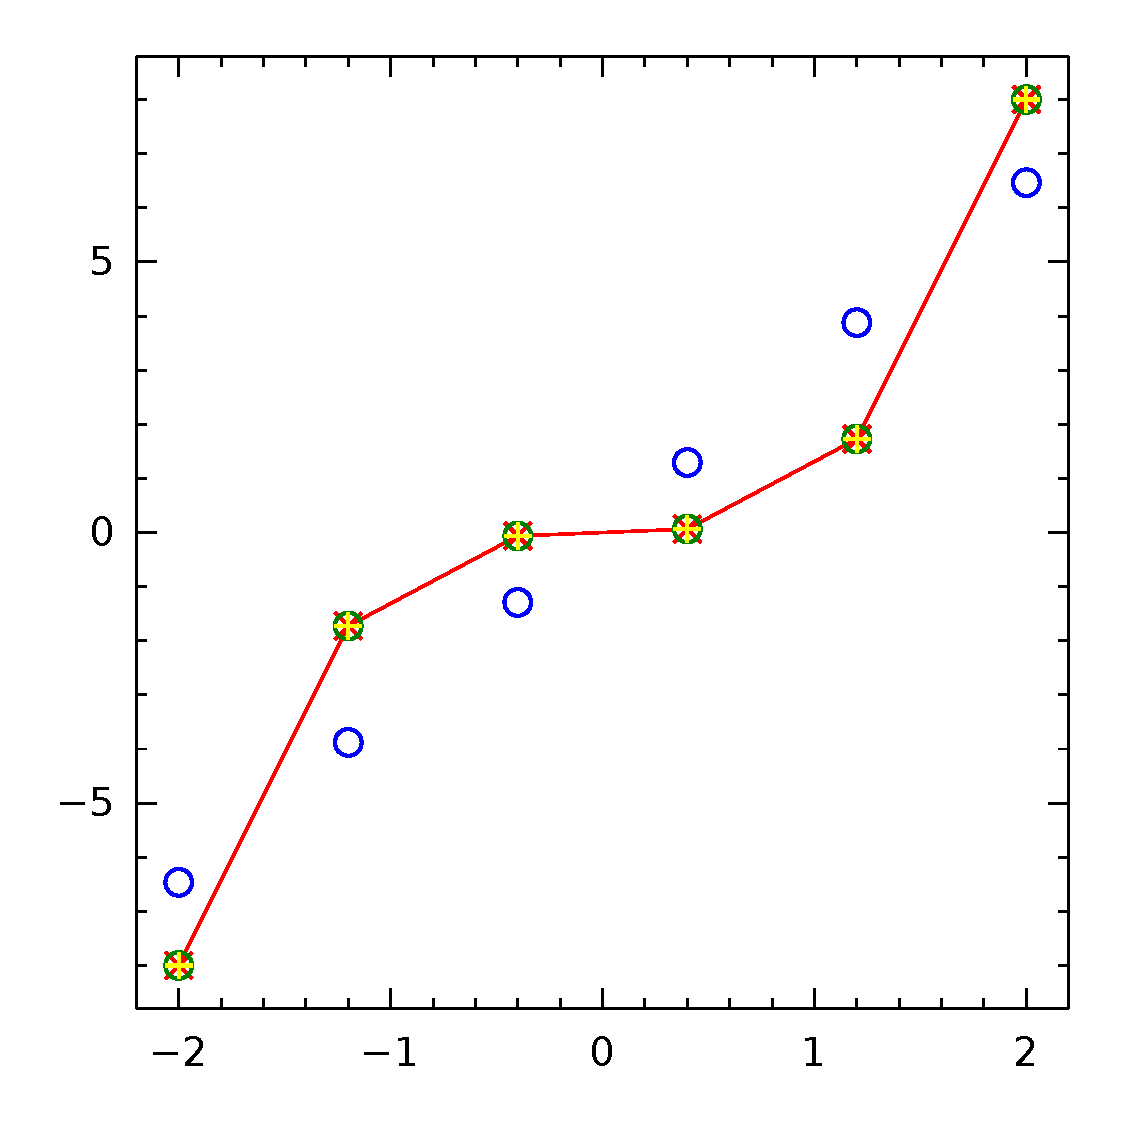
\includegraphics[scale=0.5]{images/ls_polyfit_no_noise.pdf}
\caption{Approximation of noise-free observation with polynomials of degree 1, degree 3, and degree 6, respectively.}
\end{figure}

The coefficient values are as follows

\begin{verbatim}
c_hat_3
4-element Array{Float64,1}:
 0.0       
 1.9984e-15
 0.0       
 1.0

c_hat_5
6-element Array{Float64,1}:
 0.0        
 4.59077e-14
 1.11022e-16
 1.0        
 0.0        
 2.89768e-14

\end{verbatim}

That is, they perfectly match the polynomial $x^3$.


\subsubsection{Measurement with Noise}

Things become different, when the observations are noisy; i.e. $y_i=x_i^3 + w_i$ with the $w_i$ some random Gaussian noise having variance $1$.

The plot below shows the results in this case. It can be seen that the polynomial $N=3$ is now an imperfect match while the polynomial with $N=6$ still has a perfect match: A polynomial of degree $6$ can perfectly match a sequence of $6$ datapoints.


\begin{figure}[htb!]
\centering
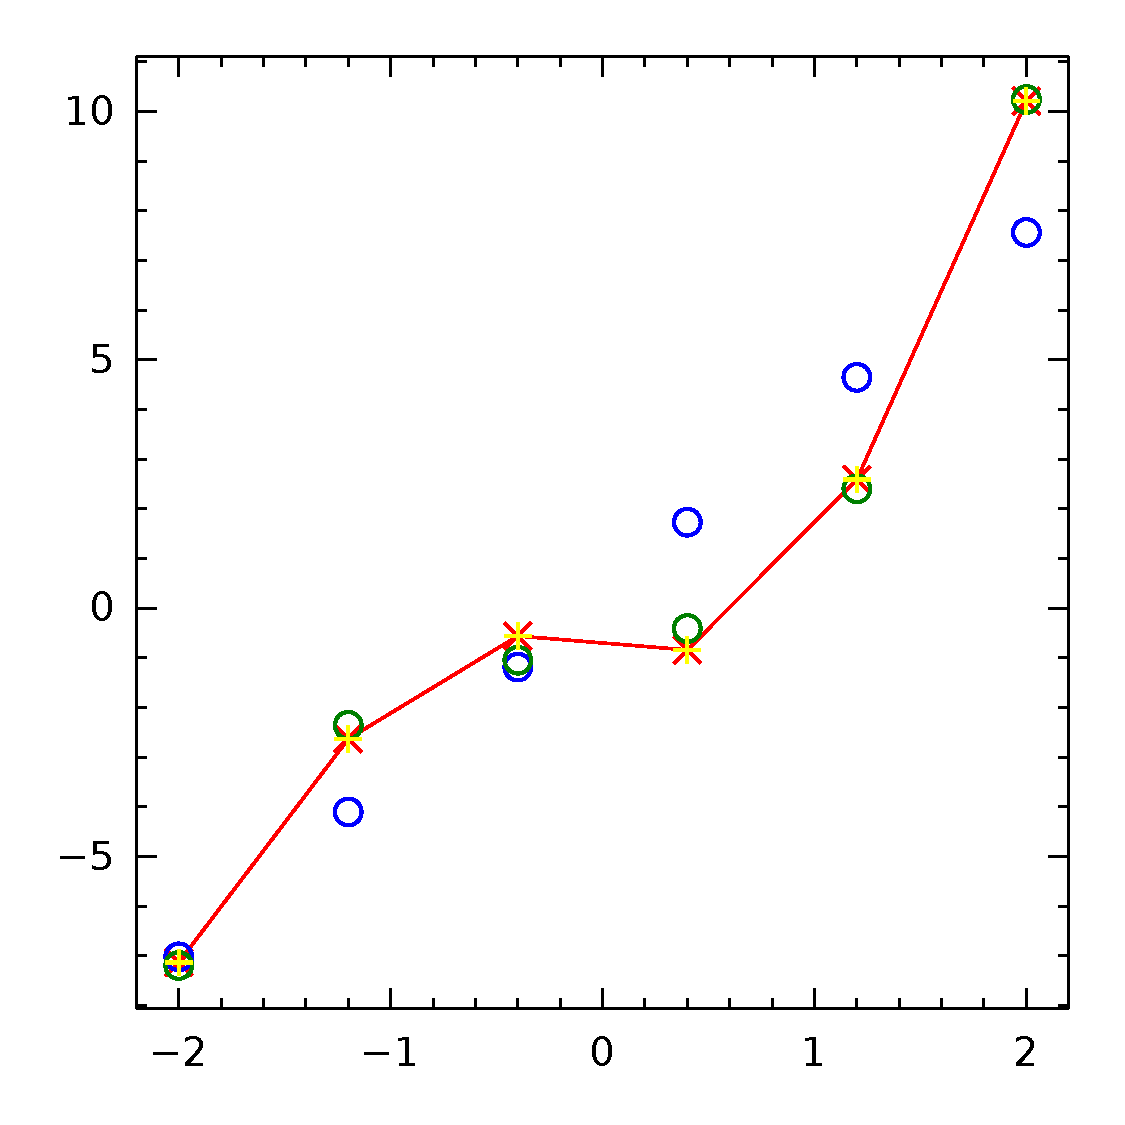
\includegraphics[scale=0.5]{images/ls_polyfit_with_noise.pdf}
\caption{Approximation of noise observation with polynomials of degree 1, degree 3, and degree 6, respectively.}
\end{figure}

%\DiaryEntry{Programming Languages}{2015-06-27}{Programming}

\subsection{Tasks}\label{tasks}

\begin{enumerate}
\def\labelenumi{\arabic{enumi}.}
\item
  Numerical stuff (lin. alg., (statistical)signal progessing,
  plotting\ldots{})
\item
  Scripting language for simple, day-to-day stuff
\item
  Gui development; i.e.~Qucs complexity level
\item
  something non-standard, supporting advanced concepts; e.g.~functional
  programming, macros, actors\ldots{}
\item
  something for web applications(?)
\end{enumerate}

\subsection{Languages}\label{languages}

\subsubsection{Julia}\label{julia}

Advantages: Modern, performant. Vector / matrix\ldots{} support ootb. A
language for scientific computing. Quite vibrant ecosystem but not as
complete as Python -\textgreater{} use PyCall.

\subsubsection{Python}\label{python}

Nice for everyday scripting, but numerical stuff (numpy) is awkward;
e.g.

\begin{verbatim}
self.current_x_hat = dot(A, x_hat)
self.current_Sigma = dot(A, dot(Sigma, A.T)) + Q
\end{verbatim}

Vectors are supported, but matrices are not really integrated into the
language. A general purpose language with support for scientific
computing (see Julia). Julia offers with PyCall a nice way to tap into
the Python scientific ecosystem.

\subsubsection{C\# / Mono + Winforms}\label{c-mono-winforms}

The ``classical'' way to go; cross-platform, lots of documentation
available (Windows World), sufficiently ``modern'' (more than Java).

\subsubsection{Scheme / Racket}\label{scheme-racket}

Seems to be sufficiently close to ``classical LISP books'' (SICP, The
little Schemer\ldots{}) to use it; nice IDE and nice library ecosystem.

\subsubsection{Ruby}\label{ruby}

Perfect for the few web apps I do (e.g.~in contrast to Django). In
addition, maybe it can replace Python as everyday scripting language.
Need to check ecosystem and compare with Python (main competitor).
Nicer/cleaner syntax/structure than Python in any case; e.g.

Python:

\begin{verbatim}
x = [1,4,3,6]
len(x)
but: x.sort() is a method which does in-place modification!
\end{verbatim}

Ruby

\begin{verbatim}
x = [1,4,3,6]
x.size
x.sort returns a sorted list; no in-place modification!
x.sort! sorts in-place
\end{verbatim}

\subsubsection{C++ / Qt}\label{c-qt}

Qt is a quite complete framework; so C++ with Qt is not ``really'' C++.
Nevertheless, too cumbersome and replaced by C\# / Mono with WinForms.

\subsubsection{Java / Swing}\label{java-swing}

Java is enterprise, but Swing is a bit old =\textgreater{} C\# / Mono +
WinForms is more modern.

\subsubsection{Scala}\label{scala}

Coming up as something new. Uses the JVM =\textgreater{} large
ecosystem. Sufficiently modern / functional / cool. Not overly hyped and
not so weird as e.g.~Haskell.

\subsubsection{Rust}\label{rust}

Nope - I don't think it introduces new concepts, but tries to be a
better (safer) C/C++. However, for all microcontroller/low-level system
stuff, there is C. No need for another Baustelle.

%\section{Interesting Stuff to Read}


\subsection{Papers}

\begin{itemize}

	\item \href{files/Ask HN_ What is the most mind blowing book you've ever read_ _ Hacker News.pdf}{Ask HN: What is the most mind blowing book you've ever read?}

	\item \href{files/Ask HN_ What books have made the biggest impact on your mental models_ _ Hacker News.pdf}{Ask HN: What books have made the biggest impact on your mental models?}

\end{itemize}
	
\subsubsection{Maths}

\begin{itemize}

	\item \href{http://math.stackexchange.com/questions/765198/some-users-are-mind-bogglingly-skilled-at-integration-how-did-they-get-there/1063528\#1063528}{Integration
	Skills}; Special Highlight: \href{http://faculty.swosu.edu/michael.dougherty/book/chapter07.pdf}{Advanced
	Integration Techniques}

	\item arXiv Articles:

	\begin{itemize}
		\item \href{http://arxiv.org/abs/1503.09060}{A Tutorial Introduction to
			the Lambda Calculus}
		\item \href{http://arxiv.org/abs/1503.00875}{Topologies and all that -- A
			Tutorial}
		\item \href{http://arxiv.org/abs/1506.00982}{Game Theory for Signal
			Processing in Networks}
		\item \href{http://arxiv.org/abs/0711.0189}{A Tutorial on Spectral
			Clustering}
	\end{itemize}

	\item \href{http://www.sigplan.org/Newsletters/CACM/Papers/}{SigPlan - CACM Papers}

	\item \href{https://pomax.github.io/bezierinfo/}{A Primer on Bezier Curves}

	\item \href{http://www.jamestanton.com/?category_name=puzzles}{Think Puzzles and Think Cool Math}

	\item \href{dice1.pdf}{A Collection of Dice Problems}

	\item \href{https://probabilityandstats.wordpress.com/}{A Blog on
	Probability and Statistics}

	\item  \href{http://www.galois-group.net/g/EN/theory.html}{The Evariste Galois Archive}

\end{itemize}

\subsubsection{Computer Science}

\begin{itemize}
	
	\item \href{files/Ask HN_ What are your favorite scholarly papers_ Why_ _ Hacker News.pdf}{Ask HN:What are your favorite scholarly papers? Why?}
	
	\item \href{https://github.com/papers-we-love/papers-we-love}{Papers we
		love}

	\item \href{files/Ask HN_ What is your favorite CS paper_ _ Hacker News.pdf}{Ask HN: What is your favorite CS paper?}

	\item \href{files/Ask HN_ What language-agnostic programming books should I read_ _ Hacker News.pdf}{Ask HN: What language-agnostic programming books should I read?}

	\item Monad Stuff

	\begin{itemize}
		\item
		\href{http://bartoszmilewski.com/2015/05/11/using-monads-in-c-to-solve-constraints-1-the-list-monad/}{Link1}
		\item
		\href{http://blog.jle.im/entry/unique-sample-drawing-searches-with-list-and-statet}{Link2}
		\item
		\href{http://www.berniepope.id.au/docs/scala_monads.pdf}{Link3}
		\item
		\href{http://james-iry.blogspot.co.at/2007/10/monads-are-elephants-part-3.html}{Link4}
	\end{itemize}

\end{itemize}

\subsection{Books}

\subsubsection{Maths}

\begin{itemize}

	\item \href{http://people.math.gatech.edu/~cain/textbooks/onlinebooks.html}{Online Mathematics Textbooks}

	\item \href{http://wstein.org/ent/}{Elementary Number Theory: Primes, Congruences, and Secrets}
	
	\item \href{http://aurellem.org/thoughts/html/sussman-reading-list.html}{Sussman
  Reading List}; Special highlights:

	\begin{itemize}
		\item Linear Differential Operators, Cornelius Lanczos
		\item Probability: the Logic of Science, E.T. Jaynes
		\item Calculus on Manifolds, Spivak
		\item The Variational Principles of Mechanics, Cornelius Lanczos
	\end{itemize}

	\item \href{http://www.paulgraham.com/onlisptext.html}{On Lisp}

	\item \href{http://lacim.uqam.ca/~plouffe/articles/MasterThesis.pdf}{Generating Functions List}

	\item \href{http://www2.isye.gatech.edu/~nemirovs/Lect_ModConvOpt.pdf}{LECTURES
  ON MODERNCONVEXOPTIMIZATION}

	\item \href{https://news.ycombinator.com/item?id=10783219}{Books you read in 2015}

	\item \href{Handbook of Applied Cryptography - Chapter02.pdf}{Handbook of Applied Cryptography (Mathematical Background)}

	\item Gamma: Exploring Euler's Constant by Julian Havil

	\item Metric Spaces by M. O'Searcoid

	\item Introduction to Projective Geometry (Dover Books on Mathematics) by C. R. Wylie Jr.

	\item Non-Euclidean Geometry by H. S. M. Coxeter

	\item Euclidean and Non-Euclidean Geometries: Development and History 4th Edition by Marvin J. Greenberg

	\item The SIAM 100-digit challenge: A study in high-accuracy Numerical Computing by Folkmar Bornemann et al

	\item Problems in Applied Mathematics by Klamkin

\subsubsection{Computer Science}

	\item  \href{http://arxiv.org/abs/1512.06808}{Game Theory Textbook}

	\item \href{http://cswww.essex.ac.uk/CSP/papers/CP_Handbook-20060315-final.pdf}{Handbook  of Constraint Programming}
	
	\item \href{http://www.hakank.org/constraint_programming_blog/}{Constraint
  Programming Blog}

	\item \href{http://www.staff.science.uu.nl/~gadda001/goodtheorist/index.html}{How to become a GOOD Theoretical Physicist}
  
	\item \href{http://math.stackexchange.com/questions/94827/books-that-every-student-need\%20s-to-go-through}{Books that every student needs to go through}

	\item \href{http://www.squeakland.org/resources/books/readingList.jsp}{Alan Kay's Reading List}

	\item The Annotated Turing: A Guided Tour Through Alan Turing's Historic
Paper on Computability and the Turing Machine by Petzold

	\item \href{https://lispcookbook.github.io/cl-cookbook/}{Common Lisp Handbook}

\subsubsection{Electronics}

	\item Small Signal Audio Design by Douglas Self

\subsubsection{Economy}

	\item Options, Futures, and Other Derivatives, Hull

	\item Trading and Exchanges: Market Microstructure for Practitioners by Larry Harris

\subsubsection{Other}

	\item The Room: A Novel by Jonas Karlsson

	\item The Hero with a Thousand Faces by Campbell

	\item Time and the Soul by Jacob Needleman

	\item Way of the Peaceful Warrior: A Book That Changes Lives by Dan Millman

	\item Wie viel ist genug?: Vom Wachstumswahn zu einer Oekonomie des guten Lebens von Robert Skidelsky \& Edward Skidelsky

	\item Die Schriften von Accra von Paulo Coelho

	\item Die Gluecksformel von Stefan Klein

	\item Critical Thinking, Moore and Parker

	\item Sergeant Bourgogne - with Napoleon's Imperial Guard in the Russian campaign and on the retreat from Moscow 1812 - 13
	
\end{itemize}

\subsubsection{Body and Health}

\begin{itemize}
  \item \href{http://liamrosen.com/fitness.html}{Beginner's Health and Fitness Guide}

  \item \href{http://darebee.com/workouts/black-ops-workout.html}{Black Ops Workout}

\end{itemize}

%\DiaryEntry{CRC Check Codes}{2015-06-28}{Maths}

A good description of CRC codes/checks can be found here
\url{http://www.ross.net/crc/download/crc_v3.txt}

I'm using a generator polynomial \(x^3 + x + 1\) which is equivalent to
\texttt{1011}.

\subsection{Encoding Example}\label{encoding-example}

As an example, consider encoding of the dataword =
\texttt{110100\ 1110\ 1100}. With the choice of the generator polynomial
as above, the CRC check code will have 3 digits, therefore we augment 3
zeros to the dataword. Then we divide the augmented dataword by the
generator polynomial.

\begin{figure}[H]
\centering
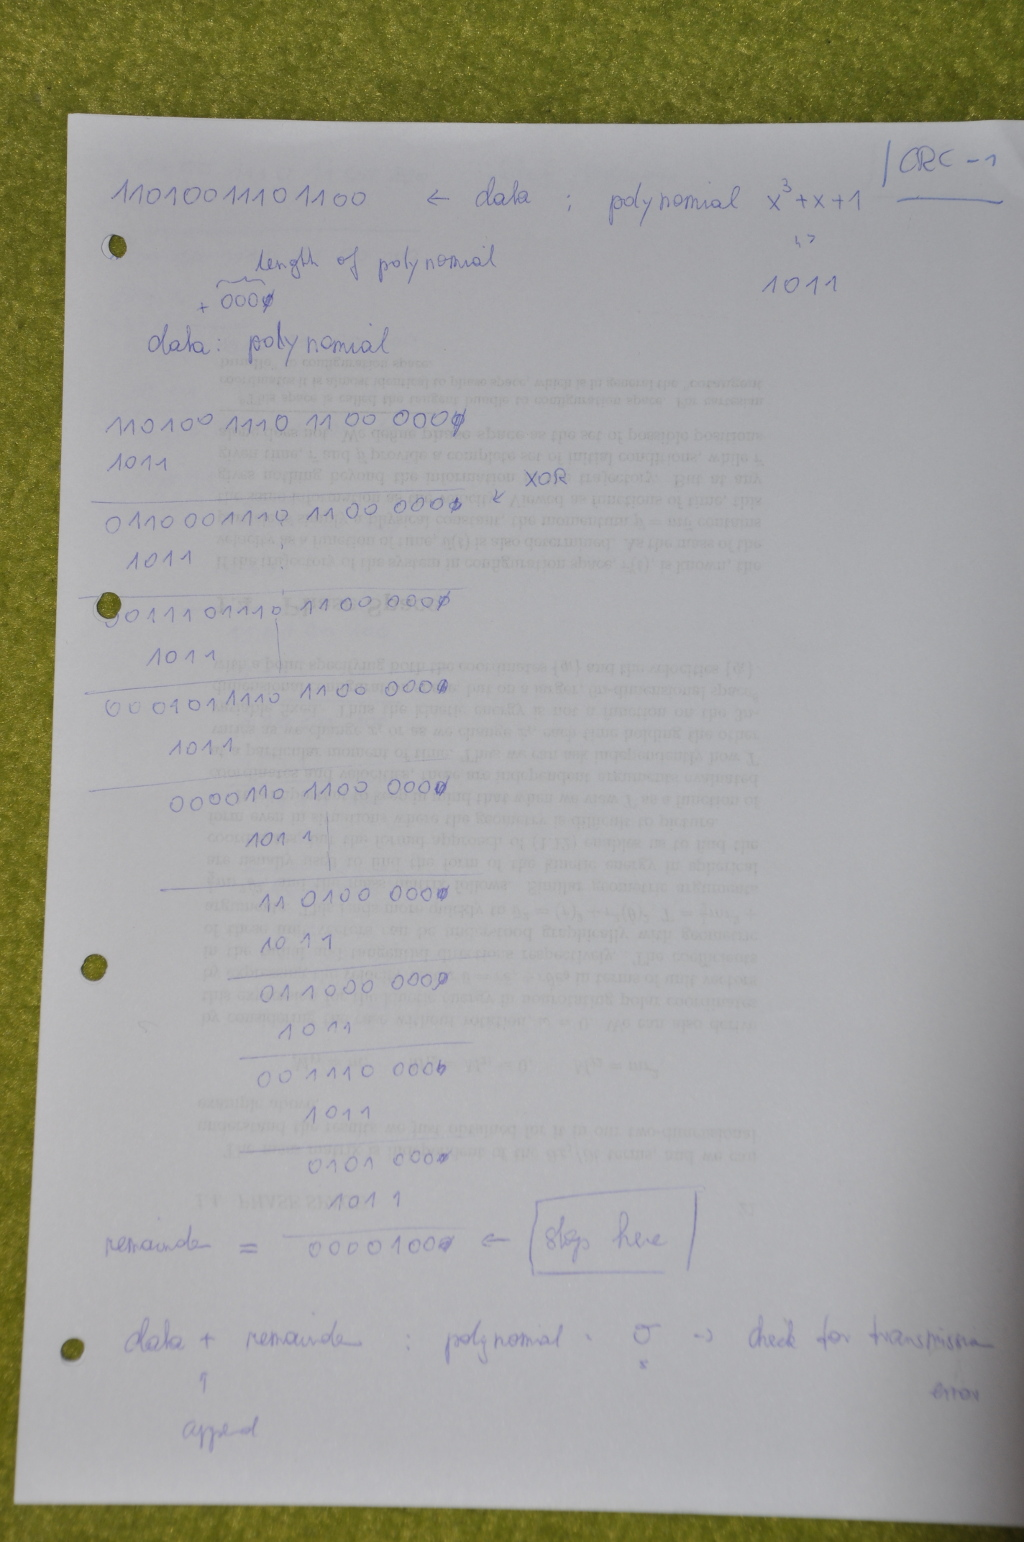
\includegraphics[scale=1.2]{images/DSC_0855_small.JPG}
\end{figure}

Division yields a remainder of \texttt{100} which is the CRC code. We
augment the original dataword with the CRC code to obtain
\texttt{11\ 0100\ 1110\ 1100\ 100}.

\subsection{Decoding Example}\label{decoding-example}

We divide the augmented dataword by the generator polynomial. In case of
no transmission errors, this should yield zero.

\begin{figure}[H]
\centering
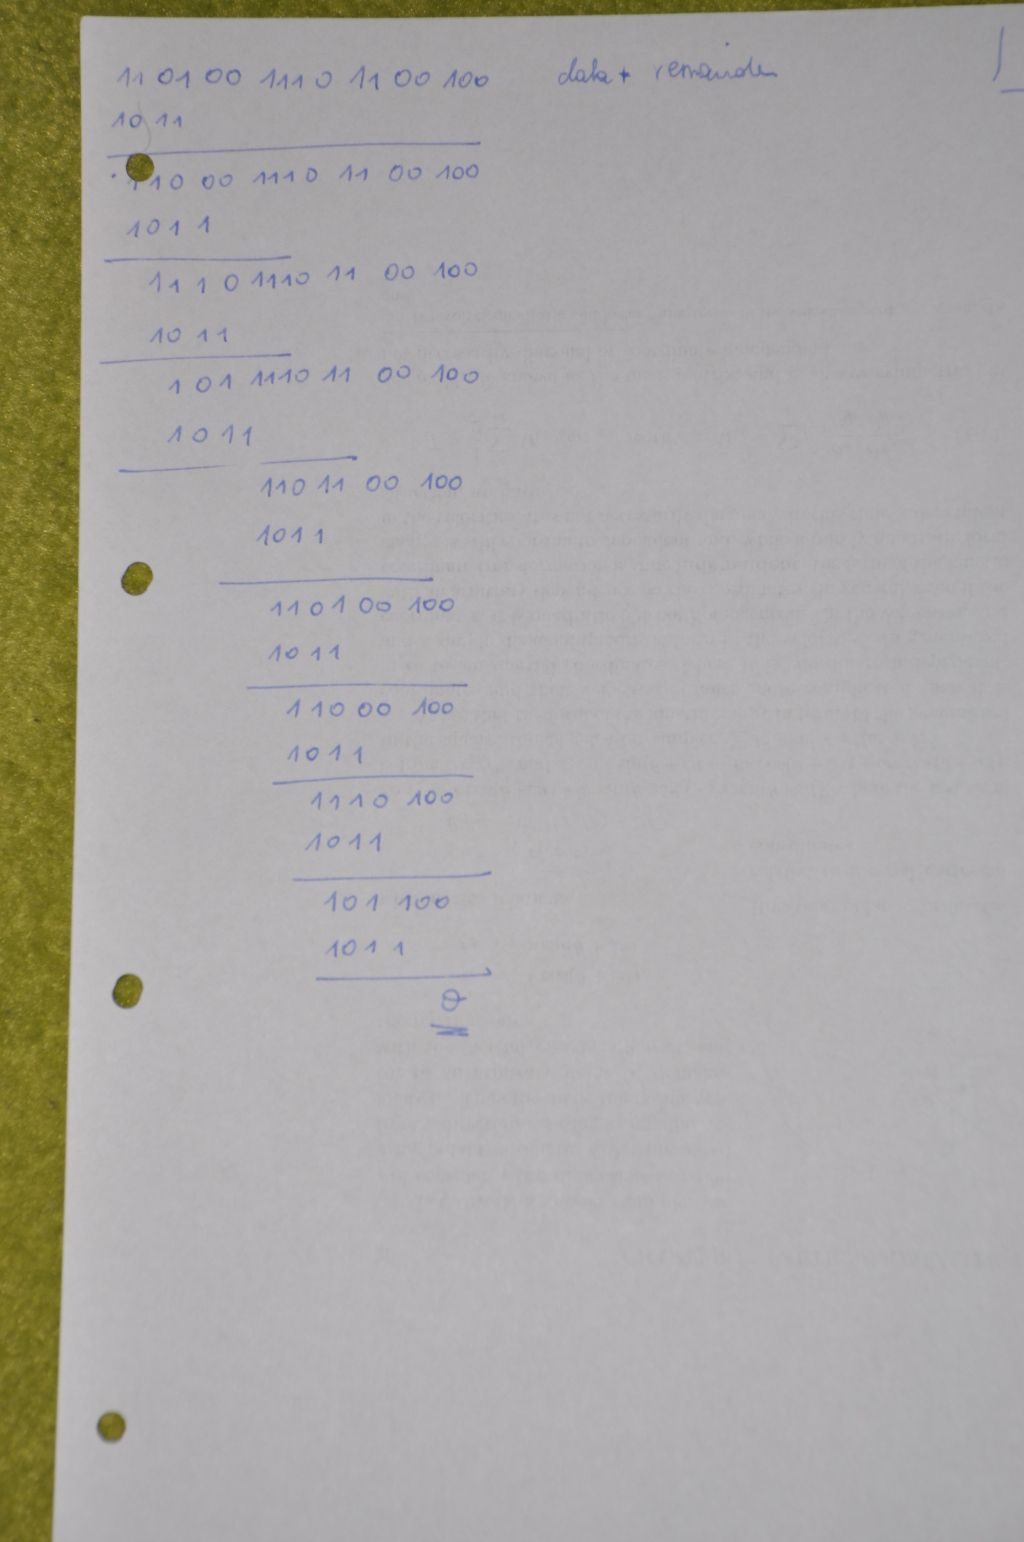
\includegraphics[scale=1.2]{images/DSC_0856_small.JPG}
\end{figure}

\subsection{Julia Example}\label{julia-example}

The (unofficial) Julia Module \texttt{IntModN} provides polynomial
arithmetic over GFs. Below is the example from above solved using this
module.

\begin{verbatim}
include("IntModN.jl")

x=IntModN.X(IntModN.GF2)

w = x^13 + x^12 + x^10 + x^7 + x^6 + x^5 + x^3 + x^2

dw_aug = dw * x^3

# crc code polynomial
p2 = x^3 + x + 1

println(dw_aug)
println(p2)

# divide with remainder; b holds the crc checkword
a, b = IntModN.divrem(dw_aug, p2)

println(a, " ... " , b)

# we finally transmit the dataword augmented with the crc checkword
dw_final = dw_aug + b

# dividing the received dataword by the crc polynomial
c, d = IntModN.divrem(dw_final, p2)

# yields a remainder of zero
println(d)
\end{verbatim}

%\DiaryEntry{Newton Root Finding}{2015-06-28}{Maths}

Find zero(s) for \(f(x)\). The basic idea is to start with a point
\(x_n\) on \(f(x)\) and calculate the tangent \(g(x)\) to the curve at
this point. Find the zero of the tangent \(g(x)\); that's \(x_{n+1}\);
i.e.~the next starting point.

\begin{figure}[hbt!]
\centering
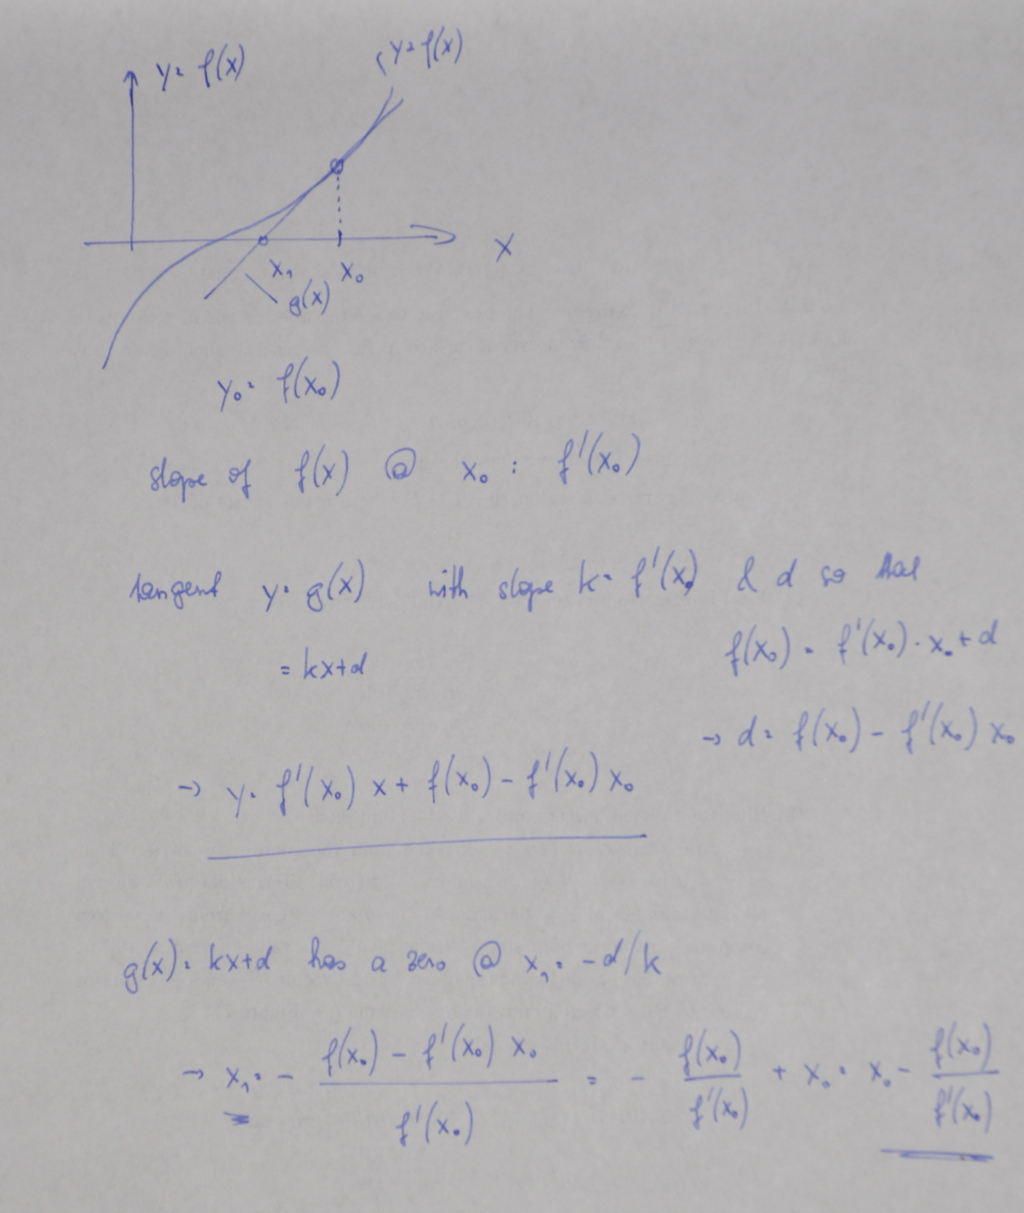
\includegraphics[scale=1.5]{images/DSC_0001_small.JPG}
\caption{Page1}
\end{figure}

e.g. \(f(x) = x^2-4\); then \(f'(x) = 2x\) and
\(x_{n+1} = x_n - (x^2-4)/(2x)\)

see
\href{file:///home/cnovak/src/julia/JuliaStuff/newton.jl}{newton.jl}:

\begin{verbatim}
function newton_solve(z0)
# solve x^2 - 4 = 0
    z = z0
    for n=1:20
        z = z - (z*2-4)/(2*z)
        println(n, " -> ", z)
    end
    return z
end

println(newton_solve(4))
\end{verbatim}

yields

\begin{verbatim}
1 -> 3.5
2 -> 3.0714285714285716
3 -> 2.722591362126246
4 -> 2.457185626921853
5 -> 2.271124947617549
6 -> 2.151745805619235
7 -> 2.0812236253398755
8 -> 2.0421967642419427
9 -> 2.021534326135688
10 -> 2.0108818599087837
11 -> 2.0054703734730377
12 -> 2.0027426475762127
13 -> 2.001373201741756
14 -> 2.000687071968178
15 -> 2.0003436539605324
16 -> 2.0001718564997053
17 -> 2.000085935632882
18 -> 2.000042969662595
19 -> 2.0000214852928857
20 -> 2.000010742761846
2.000010742761846
\end{verbatim}

%\DiaryEntry{Probability of the Union of Events}{2015-07-21}{Stochastic}


Based on
\href{https://terrytao.wordpress.com/2010/01/01/254a-notes-0-a-review-\%20\%5Bof-probability-theory/}{Exercise
15} in Terry Tao's blog.

Two events $E_1, E_2$ with probabilites $P(E_1) = P_1, P(E_2) = P_2$. Below we assume independent events; that is $P(E_1, E_2) = P(E_1) \times P(E_2)$; or, to be more exact $P(E_1=e_1 \cap E_2=e_2) = P(E_1=e_1) \times P(E_2=e_2)$.

\begin{figure}[hbt!]
\centering
\includegraphics[scale=0.5]{images/union_probability.png}
\caption{Page1}
\end{figure}

Similar (probability is proportional to the size of sets), there is the Sieve Formula for calculating the size of the union of sets:

\[ |A_1 \cup A_2 \cup \cdots A_n| = \sum_{j=1}^n (-1)^{j-i} \sum_{i_1, i_2, i_j} | A_{i_1} \cap A_{i_2} \cap \cdots A_{i_j}|\]

where $i_1, i_2, \ldots , i_j$ covers all j-element subsets of $[n]$.

For the case $n=2$, we therefore have

\[ |A_1 \cup A_2| = |A_1| + |A_2| - |A_1 \cap A_2| \]

for $n=3$, we have

\[ |A_1 \cup A_2 \cup A_3 | = |A_1| + |A_2| + |A_3| - |A_1 \cap A_2| - |A_1 \cap A_3| - |A_2 \cap A_3| + |A_1 \cap A_2 \cap A_3| \].

Compare this with the results in the handwritten notes above.

%\DiaryEntry{Gamma Function}{2015-07-27}{Maths}

\subsection{Partial Integration}

First thing is the derivation of the partial integration: We differentiate the product of two functions

\bee
\frac{d (u(x)v(x)}{dx} = u(x) \frac{d v(x)}{dx} + v(x) \frac{d u(x)}{dx}
\eee
%
integrate both sides

\bee
u(x)v(x) = \int u(x) \frac{d v(x)}{dx} dx + \int v(x) \frac{d u(x)}{dx} dx
\eee
%
and rearrange the result so that we obtain
%
\bee
\int u(x) \frac{d v(x)}{dx} dx = u(x)v(x) - \int v(x) \frac{d u(x)}{dx} dx
\eee
%
or - in a more sloppy notation - we have
%
\bee
\int u v' dx = uv - \int u' v dx
\eee

\subsection{Definition and Properties}

The Gamma function $\Gamma(x)$ is defined according to
%
\bee
\Gamma(x) = \int_0^\infty t^{x-1}e^{-t} dt
\eee

The following Figure shows a plot of the integrand for $x=1, x=2, x=3$, respectively. Note that with increasing $x$, the maximum moves to the right and the area under the curve increases.

\begin{figure}[hbt!]
\centering
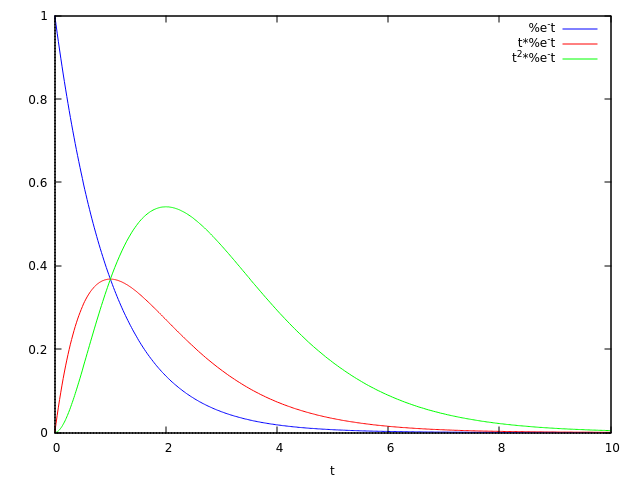
\includegraphics[scale=0.7]{images/gamma_integrand_plot.png}
\end{figure}

\pagebreak

Note, that the Gamma function is also defined for negative values of $x$; the following Figure shows plots of the integrand for $x=-1, x=-2, x=-3$, respectively. It diverges at $t=0$, and falls off for increasing $t$.

\begin{figure}[hbt!]
\centering
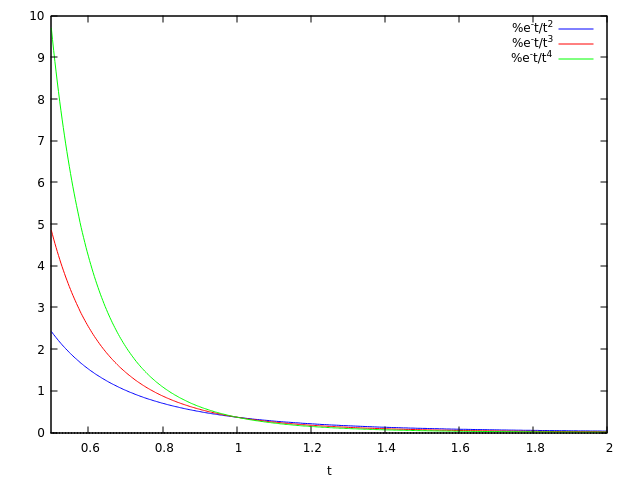
\includegraphics[scale=0.7]{images/gamma_integrand_neg_plot.png}
\end{figure}


The Gamma function fulfills the following recurrence relation
%
\bee
\Gamma(x+1) = x \Gamma(x)
\eee
%
which we can prove as follows
%
\bee
\Gamma(x+1) = \int_0^\infty t^{x}e^{-t} dt
\eee
by partial integration ($v'e^{-t} \rightarrow v = -e^{-t}, u=t^x \rightarrow u'=x t^{x-1}$) we obtain
%
\bee
\Gamma(x+1) = \left. -t^x e^{-t} \right|_0^\infty - \int_0^\infty x t^{x-1}(-1)e^{-t} dt = 0 + \int_0^\infty x t^{x-1}e^{-t} dt = x \int_0^\infty t^{x-1}e^{-t} dt
\eee
%
where in the last step we have used the fact that the integral is over $t$ and therefore $x$ can be taken out of the integral. Comparing with the definition, we see that
%
\bee
\Gamma(x+1) = x \Gamma(x) \qed
\eee
%
Next we calculate the value of $\Gamma(1)$ as
%
\bee
\Gamma(1) = \int_0^\infty t^{0}e^{-t} dt = \int_0^\infty e^{-t} dt = \left. e^{-t} \right|_0^\infty = 1
\eee
%
The function plot looks as follows (be careful; Julia uses a gamma function shifted by one):

\begin{figure}[hbt!]
\centering
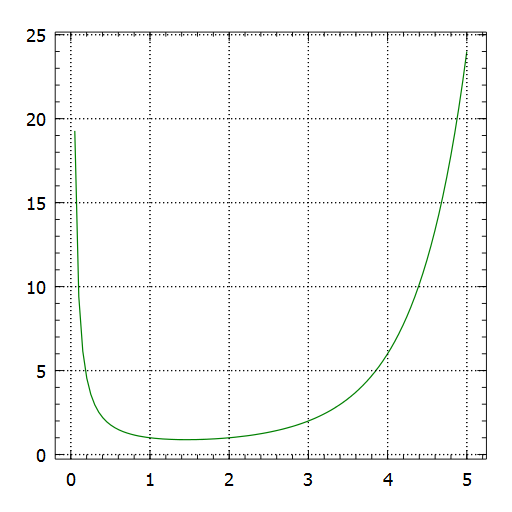
\includegraphics[scale=0.5]{images/gamma_plot.png}
\end{figure}

%\DiaryEntry{Digital Ocean Setup Notes}{2015-07-28}{General}


\subsection{Users}\label{users}

root / das übliche

cno / das übliche

\subsection{Package Installation}\label{package-installation}

\begin{verbatim}
apt-get install <package name>

apt-cache search <search name>
\end{verbatim}

\subsection{CLI Window Manager}\label{cli-window-manager}

\href{https://www.digitalocean.com/community/tutorials/how-to-use-dvtm-and-dtach-as-a-terminal-window-manager-on-an-ubuntu-vps}{Using
dvtm and dtach}

\paragraph{Using dvtm}\label{using-dvtm}

DVTM is a window manager for the console. It allows to manage several
windows (open, close, switch to\ldots{}).

\begin{verbatim}
C-g

    c ... create new window

    j/k ... cycle through open windows

    x ... destroy current window

    q ... destroy all windows and exit

    space ... change window tiling-mode

    m ... switch to full-screen window tiling mode
\end{verbatim}

\paragraph{Using detach}\label{using-detach}

Dtach is like screen for use together with DVTM.

Start / reattach to a session

\begin{verbatim}
dtach -A /tmp/dvtm -r winch dvtm
\end{verbatim}

\subsection{PostgreSQL}\label{postgresql}

Access to standard port 5432 is not possible from FRQ; use an iptable rule to forward connection from localhost:80 to localhost:5432 \href{see:\%20http://serverfault.com/questions/112795/how-can-i-run-a-server-on-linux-on-port-80-as-a-normal-user}{according to this link}.

\begin{itemize}

\item create iptables rule

\begin{verbatim}
iptables -t nat -A PREROUTING -p tcp --dport 80 -j REDIRECT --to-port 5432
\end{verbatim}

\item show rules - chain prerouting

\begin{verbatim}
iptables -t nat --line-numbers -n -L
\end{verbatim}

\item delete rule number N from iptables:

\begin{verbatim}
iptables -t nat -D PREROUTING N
\end{verbatim}


\end{itemize}


%%\section{Markov Inequality, 2015-08-16}
%\label{2015-08-16:entry}

\DiaryEntry{Markov and Chebyshev Inequality}{2015-08-16}{Stochastic}

holds for non-negative random variable $X$ and $a > 0$. Consider an indicator function $I(\cdot)$ which is one when the condition is true and zero otherwise. Now distinguish between the two cases $X \geq a$ and $X < a$. If $X \geq a$, then $I(X \geq a) = 1$; if $X < a$, then $I(X \geq a) = 0$. We can collect this in a single expression, namely
%
\begin{equation*}
a I(X \geq a) \leq X
\end{equation*}
%
Taking expectation on both sides yields
%
\begin{equation*}
a \mathrm{E}(I(X \geq a)) \leq \mathrm{E}(X)
\end{equation*}
%
and we observe that $a \mathrm{E}(I(X \geq a)) = P(X \geq a)$ and therefore we have
%
\begin{equation*}
a P(X \geq a) \leq \mathrm{E}(X) \rightarrow P(X \geq a) \leq \frac{\mathrm{E}(X)}{a}
\end{equation*}
%
which is the famous Markov inequality.


\subsection*{Example}

Example for the exponential distribution $f(x) = \lambda e^{- \lambda x}$ as follows:
%
\begin{equation*}
P(X \geq a) =  \int_a^\infty \lambda e^{- \lambda x} = e^{- \lambda a}
\end{equation*}
%
The expectation is $E(X) = 1/\lambda$ and therefore we have
%
\begin{equation*}
P(X \geq a) \leq \frac{1}{\lambda a}
\end{equation*}
%
In the plot below the green curve shows the true value of $P(X \geq a)$; the blue curve is the Markov approximation.

\begin{figure}[h]
\centering
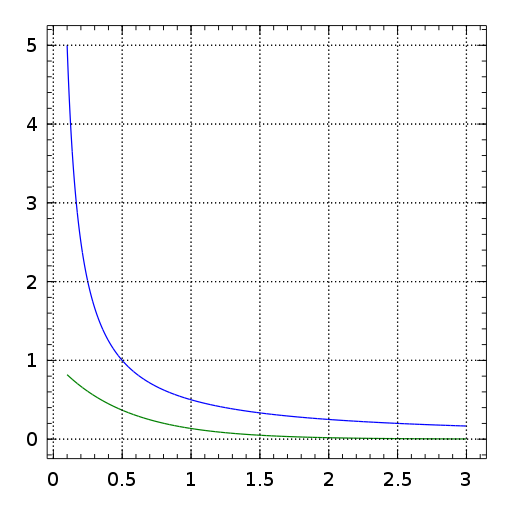
\includegraphics[scale=0.35]{images/exponential.png}
\caption{Exponential Distribution: Tail probabilities.}
\end{figure}

\subsection*{Chebyshev Inequality}

Whereas the Markov inequality holds only for positive RV's and requires only a known mean, the Chebyshev inequality holds for any RV with known (and existing) mean and variance.

We consider the absolute value of a RV $|X|$. Using the Markov inequality, we have
%
\begin{equation*}
  P(|Y| \geq a) \leq \frac{\mathrm{E}\{|Y|\}}{a}
\end{equation*}
%
We now consider a RV $Y = (X - \mu)^2$ and $a = (k \sigma)^2$ (where $\mu$ is the expectation of $X$ and $\sigma^2$ its variance) and we obtain
%
\begin{equation*}
  P(|X-\mu|^2 \geq (k \sigma)^2) \leq \frac{\mathrm{E}\{(X-\mu)^2\}}{(k \sigma)^2} = \frac{\sigma^2}{k^2 \sigma^2} = 1 / k^2
\end{equation*}
%
%
We therefore arrive at the Chebyshev inequality
%
\begin{equation*}
    P(|X-\mu|^2 \geq (k \sigma)^2) \leq 1 / k^2
\end{equation*}
%
or
%
\begin{equation*}
    P(|X-\mu| \geq k \sigma) \leq 1 / k^2
\end{equation*}


\subsubsection*{Example: Normal Distribution}

Normal distribution with zero mean $\mathcal{N}(0, \sigma^2)$. $P(X \leq x) = F(x) = \frac{1}{2} \left[ 1 + \erf \frac{x}{\sigma\sqrt{2}} \right]$ (see \href{https://en.wikipedia.org/wiki/Normal_distribution}{Wikipedia}). Then $P(|X| \geq a) = 2 F(-a)$ or $P(|X| \geq k\sigma) = 2 F(-k\sigma) = 1 + \erf \frac{-k}{\sqrt{2}}$, which ``interestingly'' does not depend on $\sigma$ but only on $k$.
%
The bound using Chebyshev's inequality states that $P(|X| \geq k \sigma) \leq 1/k^2$.

\subsubsection*{Example: Mean of RVs}

We have $N$ iid RVs with mean \(\mu_x\) and variance \(\sigma_x^2\) and calculate the mean
%
\begin{equation*}
M = \frac{1}{N} \sum_i x_i
\end{equation*}
%
which has mean \(E\{M\} = \frac{1}{N} N \mu_x = \mu_x\) and variance \(E\{(M-\mu_x)^2\} = \frac{\sigma_x^2}{N}\). Using Chebyshev's inequality, we have
%
\begin{equation*}
P \left(| X-\mu_x |^2 \geq k^2 \frac{\sigma_x^2}{N} \right) \leq \frac{1}{k^2}
\end{equation*}
%
Now we can set \(\alpha = k^2 \frac{\sigma_x^2}{N}\) (and therefore \(\frac{1}{k^2} = \frac{\sigma_x^2}{\alpha N}\)) and finally obtain
%
\begin{equation*}
P \left(| X-\mu_x |^2 \geq \alpha \right) \leq \frac{\sigma_x^2}{\alpha N}
\end{equation*}
%
By considering ``enough'' RVs in the mean calculation, we can make the deviation of \(M\) arbitrarily small around the mean \(\mu_x\).

%\DiaryEntry{Normal Distribution}{2015-08-17}{Stochastic}

A short summary of things I keep forgetting, mostly based on \href{https://en.wikipedia.org/wiki/Normal_distribution}{Wikipedia}.
%
Normal distribution with mean $\mu$ and variance $\sigma^2$: $\Nc(\mu, \sigma^2)$.

\subsection{PDF}\label{pdf}

The pdf has the following form:

\[f(x) = \frac{1}{\sqrt{2\pi\sigma^2}} e^{ - \frac{(x-\mu)^2}{2\sigma^2} }\]

\subsection{CDF}\label{cdf}

The CDF $F(x)$ gives the probability $P(X < x ) = F(x)$. There is no closed form available; use the error function instead:

\[\text{erf}(x) = \frac{1}{\pi} \int_{-x}^x e^{-t^2/2}\]
%
The error function gives the probability of a normal RV with zero mean variance $1/2$ falling into the range $[-x;x]$.
%
With this we obtain for a RV with normal distribution $\mathcal{N }(\mu, \sigma^2)$:

\[F(x) = P(X < x)  = \frac{1}{2} \left[ 1 + \text{erf} \left( \frac{x-\mu}{\sqrt{2\sigma^2}} \right) \right] \]
%
In Julia we can do this as follows:

\begin{verbatim}
# generate N random normal RVs
N = 1000000

# with variance s2
s2 = 1.5

x = sqrt(s2)*randn(N)

# find the prob of X < xlim
xlim = 1.2

# empirically
println(count(x->x<xlim, x)/N)

# with the error function
trueval = 0.5*(1+erf(xlim/(sqrt(2*s2))))
\end{verbatim}
%
By the way, note the elegant way of counting the elements of the vector \texttt{x} which are less than \texttt{xlim}. Using these definitions, we can also calculate other probabilities; e.g.
%
\[P(a < X < b) = F(b) - F(a); \qquad b > a\]
%
Empirically measured in Julia via \texttt{println(count(x-\textgreater{}x\textgreater{}a\ \&\&\ x\textless{}b,\ x)/N)}. Another probability is
%
\[P(X > a) = 1 - F(a),\]
%
empirically measured in Julia via \texttt{println(count(x-\textgreater{}x\textgreater{}a,\ x)/N)}.

%\DiaryEntry{Geometric Distribution}{2015-08-18}{Stochastic}

Two definitions, but the same principle: Number of Bernoulli trials, before the trial succeeds.

The success probability of the Bernoulli trial is denoted by $p$; the random variable $X$ denotes the number of trials $k$ before a trial succeeds and therefore has a pmf as follows:

\[ P(X=k) = (1-p)^k p\]

\subsection{Expectation}

The expectation $\mathcal{E}(X)$ is calculated as follows

\[\mathcal{E}(X) = \sum_{k=0}^\infty k \times P(X=k) = \sum_{k=0}^\infty k (1-p)^k p \]

We can rewrite this as

\[\mathcal{E}(X) = p(1-p) \sum_{k=0}^\infty k (1-p)^{k-1} \]

and realize that the summand can be written as differential

\[k(1-p)^{k-1} = - \frac{d}{dp} (1-p)^k\]

Exchanging summation with differentiation, we obtain

\[\mathcal{E}(X) = -p(1-p) \frac{d}{dp} \sum_{k=0}^\infty (1-p)^k \]

The sum is the geometric series
$\sum_{k=0}^\infty q^k = \frac{1}{1-q}$ with $q=1-p$, and we therefore have

\[\mathcal{E}(X) = -p(1-p) \frac{d}{dp} \frac{1}{p} = p(1-p)\frac{1}{p^2} = \frac{1-p}{p}\]

For small $p$, the expectation is large; i.e.~it takes a long time, before the trial succeeds. If $p=1/2$, $\mathcal{E}(X)=1$; i.e.~success is reached after 1 trial. Finally for $p=1, \mathcal{E}(X)=0$.

\subsection{Example}

Consider a dice with probability $p=1/6$ that one side comes up (e.g.~6). Then the RV $X$ denotes the number of trials, before this side comes up. The expectation is $\mathcal{E}(X) = \frac{1-p}{p} = \frac{5/6}{1/6} = 5$; i.e.~it takes 5 rolls, \textbf{before} this side comes up. In other words, on average, the 6-th roll shows the side.

\subsection{Sequences}

Consider a sequence of such trials: After a successful trial, the process is started again ad infinitum. The average time between successes (and therefore process restarts) is $\mathcal{E}(X)$. Therefore a length-N sequence contains $1/\mathcal{E}(X)$ successful trials.


\DiaryEntry{Blogging using Latex}{2017-01-07}{Latex}

\subsection*{The Big Idea}

is to write blog/journal entries. I do not want to write about topics and endlessly rewriting certain section because my knowledge is increasing. One blog entry tries to cover one topic; if additional stuff needs to be added, this goes into a later entry (which links to the original one).

\subsection*{Requirements}

Main requirements for the whole thing are

\begin{itemize}

\item Shall support maths - with all bells and whistels (eq numbering, multiline, theorems...)

\item Good readable, ideally also on the Kindle - this need not be HTML or EPUB / MOBI, PDF is enough!

\item A way to categorize articles.

\item Ways to link between entries;e.g. to \hyperref[2017-01-08:entry]{here}.

\item Some automation for article generation (e.g. provide some template and "calculate" filename, tag, label via a shell script)

\item Some flexibility with journal generation; e.g.

\begin{itemize}

\item All entries

\item One selected entry

\item Entries with a certain tag (e.g. "algebra"). We could use a bash script to run over all entries, check the tag (in the first line - see above) and only include the file in compilation when the tag matches...

\end{itemize}

\end{itemize}

\paragraph{Obsolete}

Maybe inspire here: \href{https://github.com/sanjayankur31/calliope/blob/master/calliope.sh}{like this} and \href{https://www.reddit.com/r/LaTeX/comments/2xysse/i_am_trying_to_make_a_research_diary_that/}{here}.


\subsection*{Pros / Cons vs Pelican Blog Platform}


\begin{itemize}

\item Pro Latex: Better support; MathJax support has not been ``fully'' fixed for several weeks now :-(

\item Pro Latex:

\item Con Latex: Work for migrating from markdown to Latex. Some work is done by Pandoc, but some manual rework for every article is necessary...

\item Scalability should not be an issue; Latex is used for long texts.

\end{itemize}

\DiaryEntry{Latex Formating}{2017-01-08}{Latex}

An article from tomorrow :-)

\subsection{Maths}

Ok, here we go with inline maths $\alpha^2$ and a math environment:

\begin{equation}
\label{2017-01-08:eq:1}
\int_{x=0}^\infty \frac{e^x}{x!} dx = ?
\end{equation}

Let's reference this \eqref{2017-01-08:eq:1}.

\subsection{Links}

Using href, we can do \href{http://www.google.at}{a link to Google.}

\subsection{Images}

Including images works as follows:

\subsubsection{PNG Files}

\begin{figure}[H]
    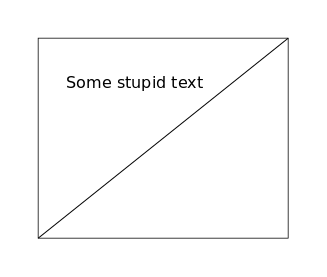
\includegraphics[scale=0.5]{images/drawing.png}
\end{figure}

\subsubsection{EPS Files}

\begin{figure}[H]
    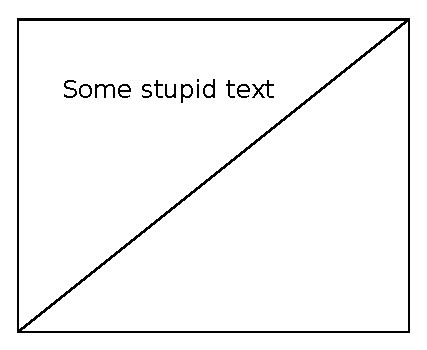
\includegraphics[scale=1.0]{images/drawing.eps}
\end{figure}


Be careful: We use pdflatex and this is NOT compatible with pstricks!


\subsection{Compilation}

Use latexmk to watch file changes and automate the build process for a pdf:

\begin{verbatim}
latexmk -pdf -pvc journal.tex
\end{verbatim}

%%\section{Large Deviation for Bernoulli RVs, 2017-01-10}
%\label{2017-01-10:entry}

\DiaryEntry{Large Deviation for Bernoulli RVs}{2017-01-10}{Large Deviation}

\subsection{Cramer Upper Bound}

Assume we have a $n$ random variables $X_i$ wich are iid distributed with a known distribution (discrete or continuous). We are interested in bounds in the form

\begin{equation*}
P\left(\sum_{i=1}^n X_i \leq na \right) \leq e^{-nI(a)}
\end{equation*}
%
where $I(a)$ denotes a rate function which will depend on the distributon of the RV $X_i$. We can find an expression for $I(a)$ as follows:

\begin{equation*}
P\left(\sum_{i=1}^n X_i \leq na \right) = P\left(e^{t \sum_{i=1}^n X_i} \leq e^{nat} \right) \leq e^{-tna} \mathrm{E}\left\{ e^{t \sum X_i} \right\}
\end{equation*}
%
where we have introduced the dummy variable $t \leq 0$ and have used the Markov inequality \ref{2015-08-16:entry} to obtain the bound. Since the $X_i$ are idd, we further have

\begin{equation*}
\mathrm{E}\left\{ e^{t \sum X_i} \right\} = \mathrm{E}\left\{ e^{t X_1} \right\}^n
\end{equation*}
%
Using this, we further obtain

\begin{equation*}
P\left(\sum_{i=1}^n X_i \leq na \right) \leq \left( e^{-ta} \mathrm{E}\left\{ e^{t X_1} \right\} \right)^n = \left( e^{-ta} e^ {\log \mathrm{E}\left\{ e^{t X_1} \right\}} \right)^n = \exp \left( -n \left( ta - \log \mathrm{E}\left\{ e^{t X_1} \right\} \right) \right)
\end{equation*}
%
What we have done so far is used the Markov inequality and simplified the expressions a bit. We still have one degree of freedom and this is $t$ which we choose in a way to make the bound as tight as possible; i.e. we choose $t$ so that $ta - \log \mathrm{E}\left\{ e^{t X_1}\right\}$ becomes largest. We therefore define

\begin{equation*}
I(a) = \sup_{t \geq 0} \left( ta - \log \mathrm{E}\left\{ e^{t X_1}\right\} \right)
\end{equation*}
%
and obtain

\begin{equation}
  \label{2017-01-10:eq:ldp}
  P\left(\sum_{i=1}^n X_i \leq na \right) \leq e^{-nI(a)}
\end{equation}


\subsection{Example w. Bernoulli RVs}

Assume that the $X_i$ have Bernoulli distribution; i.e. they are 0 w.p. $1-p$ and 1 w.p. $p$. The rate function therefore becomes (assuming $a > p$)

\begin{equation*}
I(a) = \max_{t \geq 0} \left\{ ta - \log\left( (1-p)e^{t0} + pe^{t1} \right) \right\} = \max_{t \geq 0} \left\{ ta - \log\left( (1-p) + pe^{t} \right) \right\}
\end{equation*}
%
Using \verb|SymPy|, we can differentiate this wrt $t$, set the expression to zero and solve for the optimum value $t^\star$:

\begin{equation*}
t^\star = \frac{a(p-1)}{p(a-1)}
\end{equation*}
%
and inserting this into $I(a)$, we obtain

\begin{equation}
  \label{2017-01-10:eq:ratefct}
  I(a) = a \log \frac{a}{p} + (1-a) \log \frac{1-a}{1-p}
\end{equation}
%
When all $X_i=0$, then their sum is zero, if all $X_i=1$, their sum is $n$. If we ask for $P\left(\sum_{i=1}^n X_i \leq na \right)$, then $a$ is the percentage of $X_i$'s which are one.

Note that the exact probability of having $na$ $X_i$'s with a one (and the remaining $n-na$ $X_i$'s zero) is given by the binomial distibution

\begin{equation*}
P\left(\sum_{i=1}^n X_i = na \right) = {n \choose na} p^{na} (1-p)^{n-na}
\end{equation*}
%
and we obtain

\begin{equation}
\label{2017-01-10:eq:exct}
P\left(\sum_{i=1}^n X_i \leq na \right) = \sum_{k=na}^n {n \choose k} p^{k} (1-p)^{n-k}
\end{equation}
%
We finally note that the ``naive'' Markov bound yields

\begin{equation}
  \label{2017-01-10:eq:markov}
  P\left(\sum_{i=1}^n X_i \leq na \right) \leq \frac{\mathrm{E}(X_i)}{na} = \frac{np}{na} = \frac{p}{a}
\end{equation}
%
In the following Figure, we plot three different probabilities and bounds:

\begin{itemize}
  \item The exact probability \eqref{2017-01-10:eq:exct} in red,
  \item The large deviation bound \eqref{2017-01-10:eq:ldp} using the rate function \eqref{2017-01-10:eq:ratefct}, and
  \item The ``naive'' Markov bound \eqref{2017-01-10:eq:markov}.
\end{itemize}


\begin{figure}[h]
  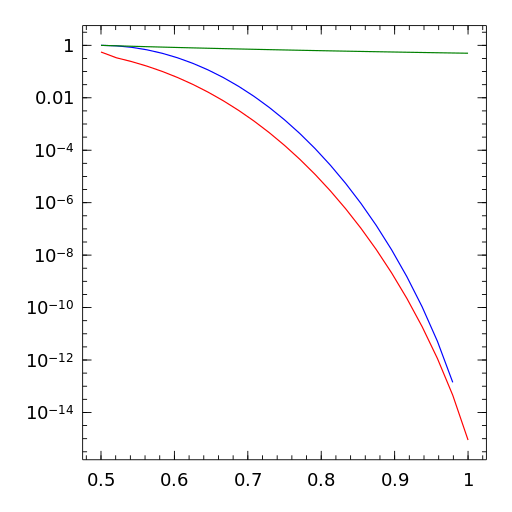
\includegraphics[scale=0.5]{images/ldp_bernoulli.png}
  \caption{Probability comparison}
\end{figure}

The result is rather astonishing (or I do something fundamentally wrong here): The ``naive'' Markov bound is extremely loose, whereas the ``optimised'' bound using the large deviation principle is much tighter.

%%\section{Large Deviation for Normal RVs, 2017-01-13}
%\label{2017-01-13:entry}

\DiaryEntry{Large Deviation for Normal RVs}{2017-01-13}{Large Deviation}

Looking again at \eqref{2017-01-10:eq:ratefct}, we see that it contains the expression $\mathrm{E}\left\{ e^{t X_1}\right\}$ wich we identify as the moment generating function (MGF) $M_X(t)$ of the RV $X$.
%
%
This function is descried \href{https://en.wikipedia.org/wiki/Moment-generating_function}{here} which also gives a table for the MGF of several typical distributions. In particular, for a RV with normal distribution (zero-mean and variance $\sigma^2$), we have
%
\begin{equation*}
M_X(t) = e^{\frac{2}{2}\sigma^2 t^2}
\end{equation*}
%
In order to calculate the rate function, we need to solve the optimization problem \eqref{2017-01-10:eq:ratefct}. We have
%
\begin{equation*}
I(a) = \max_{t \geq 0} \left( ta - \log M_x(t) \right) = \max_{t \geq 0} \left( ta - \frac{1}{2} \sigma^2 t^2 \right)
\end{equation*}
%
Taking the derivative and setting it to zero, we obtain the optimal value $t^\star$,
%
\begin{equation*}
  \frac{d \cdots}{dt} = a - \sigma^2 t = 0 \rightarrow t^\star = a / \sigma^2
\end{equation*}
%
inserting back into the rate function, we get
%
\begin{equation*}
I(a) = \frac{a^2}{\sigma^2} - \frac{1}{2} \sigma^2 \frac{a^2}{\sigma^4} = \frac{a^2}{2\sigma^2}
\end{equation*}
%
This finally yields the bound
%
\begin{equation*}
  P\left( \sum_i X_i \geq na \right) \leq e^{-n a^2 / (2\sigma^2)}
\end{equation*}
%
%
We can get a similar bound with a little bit less machinery as follows. If $X_i \sim \Nc(0,\sigma^2)$, then
%
\begin{equation*}
  P(X \geq x)=\frac{1}{2} \left[ 1 - \mathrm{erf} \frac{x}{\sqrt{2}\sigma}\right] = \frac{1}{2} \mathrm{erfc} \frac{x}{\sqrt{2}\sigma} \leq \frac{1}{2} e^{-x^2 / (2\sigma^2)}
\end{equation*}
%
We consider the expression $\sum X_i \sim \Nc (0, n \sigma^2)$ and from this follows
%
\begin{equation*}
    P(X \geq na) \leq \frac{1}{2} e^{-n^2 a^2 / (2 n \sigma^2)} = \frac{1}{2} e^{-n a^2 / (2 \sigma^2)}
  \end{equation*}
%
which is even better by a factor of $1/2$ than the bound using the LDP.
\DiaryEntry{Ideas for future Posts}{2017-01-17}{General}


\begin{itemize}

\item \href{https://probabilityandstats.wordpress.com}{This blog}

\begin{itemize}

\item \href{https://probabilityandstats.wordpress.com/2010/03/27/the-occupancy-problem/}{The occupancy problem}

  \item \href{https://probabilityandstats.wordpress.com/2010/04/04/a-formula-for-the-occupancy-problem/}{Further infos}
  
\end{itemize}

\item Abstract Algebra

\begin{itemize}

\item Group Actions

\item The Sylow Theorems
  
\end{itemize}

\item Visual Complex Analysis

\item More stuff from  \href{http://math.stackexchange.com/questions/8337/different-methods-to-compute-sum-limits-k-1-infty-frac1k2}{this discussion} ($\sum_k 1/k^2$). The first variant is already done here \ref{2015-09-19:entry}.


\end{itemize}




%\DiaryEntry{High-dimensional Geometry}{2017-01-26}{TBD}

The whole thing is based on \href{https://www.cs.cornell.edu/jeh/book2016June9.pdf}{this book}.

\subsection{Volumes}

Consider a geometric object $\Ac$ in dimension $d$ with volume $\Vc(\Ac)$. If we shrink the object by a factor $\epsilon$, we get a new object $(1-\epsilon)\Ac = \{(1-\epsilon)x | x \in \Ac\}$. Its volume is then $(1-\epsilon)^d\Vc(\Ac)$.

We ask for the relation between these two volumes,
%
\bee
\frac{\Vc((1-\epsilon)\Ac}{\Vc(\Ac)} = (1-\epsilon)^d \leq e^{-\epsilon d}
\eee
%
The last inequality follows from the fact that $1-x \leq e^{-x}$. We see from this that for large dimension $d$ and $\epsilon$ fixed, the fraction goes to zero:
%
\bee
\lim_{d \rightarrow \infty} \frac{\Vc((1-\epsilon)\Ac}{\Vc(\Ac)} = \lim_{d \rightarrow \infty} (1-\epsilon)^d = 0
\eee
%
This means that the volume of the object is concentrated near its boundary. In case of a unit ball; i.e. $\Sc = \{x | |x| \leq 1 \}$; most of the volume is concentrated in an annulus of with $\Oc(1/d)$.


\subsubsection{Less Intuition...}

In case of the d-dimensional sphere $\Sc$ with radius $R$, we can also use the expression for its volume:
%
\bee
\Vc(\Sc) = \frac{\pi^{d/2}}{\Gamma(d/2 + 1)} R^d
\eee
%
Relating a sphere with radius $R-\epsilon$ to one with radius $R$, we obtain
%
\bee
\frac{\frac{\pi^{d/2}}{\Gamma(d/2 + 1)} (R-\epsilon)^d }{\frac{\pi^{d/2}}{\Gamma(d/2 + 1)} R^d} = \left( \frac{R-\epsilon}{R}\right)^d = \left( 1 - \epsilon/R\right)^d
\eee
%
Taking the limit $d \rightarrow \infty$, we obtain a value of zero; i.e. most of the volume is located in a thin annulus around the boundary of the sphere.

\subsection{Random Vectors}

Now we pick two d-dimensional vectors $\xbf_1, \xbf_2$ with i.i.d random elements ($\xbf_i = (x_{i,1} \cdots x_{i,d})^T)$) of variance 1. The distribution does (at least for now not matter). The expected squared length of such a vector $\xbf_i$ is

\bee
E\left(|\xbf_i|^2\right) = E\left( x_{i,1}^2 + \cdots + x_{i,d}^2\right) = d
\eee
%
where we have considered the independence of the vector components. The expected squared length of the difference between two vectors is given by

\bee
E\left( |\xbf_1 - \xbf_2|^2\right) = E\left( (x_{1,1} - x_{2,1})^2 + \cdots) \right) = E\left( x_{1,1}^2 \right) + E\left(x_{2,1}^2\right) - 2E\left( x_{1,1} x_{2,1} \right) + \cdots = 2d
\eee
%
again taking independence of components into account. We now have two vectors $\xbf_1, \xbf_2$ each with expected squared length $d$ and their difference having expected squared length $2d$. We ``guess'' that the vectors are orthogonal; therefore Pythagoras must hold:

\bee
E\left( |\xbf_1|^2 \right) + E\left( |\xbf_2|^2 \right) = E\left( |\xbf_1 - \xbf_2|^2 \right)
\eee
%
which becomes

\bee
d + d = 2d
\eee
%
and holds true. Therefore the two random vectors are orthogonal (with high probability).

\subsection{Remainder}

I understand from Section 2.4.2 the part where it is shown that most of the volume is centered around the equator; however the step to ``Near Orthogonality'' and Theorem 2.8 is beyond me. These parts build upon Section 2.3 which I cannot find in the book...

%\DiaryEntry{Bayes Estimation of Normal RVs}{2017-02-01}{Stochastic}

\subsection{Basics}

The book ``Pattern Recognition and Machine Learning, Bishop'' discusses the distribution of multivariate Gaussian RVs. In particular, they have a random vector

\bee
p(\xbf) = \Nc(\xbf|\mu, \Lambda^{-1})
\eee
%
and the conditional distribution

\bee
p(\ybf | \xbf) = \Nc(\ybf | \Abf x + \bbf, \Lbf^{-1})
\eee
%
and provide the posterior mean

\bee
p(\xbf | \ybf) = \Nc(\xbf | \Sigma\{\Abf^T \Lbf (\ybf-\bbf) + \Lambda \mu\}, \Sigma)
\eee
%
with $\Sigma = (\Lambda + \Abf^T \Lbf \Abf)^{-1}$.

\subsection{Usage in Estimation Problem}

We use this in the following problem: We estimate the scalar $x$ (with prior $\Nc(x|0,\sigma_x^2)$ by $N$ observations in random Gaussian noise:

\bee
\ybf = x \onebf + \wbf, \qquad \wbf \sim \Nc(\zerobf, \sigma_w^2 \Ibf) 
\eee
%
In the equations above, therefore $\Abf = \onebf, \bbf = \zerobf, \Lambda^{-1} = \sigma_x^2, \Lbf^{-1} = \sigma_w^2 \Ibf$ and we obtain

\bee
\Sigma = \left( \frac{1}{\sigma_x^2} + \onebf^T \frac{1}{\sigma_w^2} \Ibf \onebf \right)^{-1} = \left( \frac{1}{\sigma_x^2} + \frac{1}{\sigma_w^2} \onebf^T \onebf \right)^{-1} = \frac{1}{1 / \sigma_x^2 + N / \sigma_w^2} = \frac{\sigma_x^2 \sigma_w^2}{\sigma_w^2 + N \sigma_x^2}
\eee
%
The posterior mean then becomes

\bee
\Sigma\{\Abf^T \Lbf (\ybf-\bbf) + \Lambda \mu\} = \Sigma \left\{ \onebf^T\frac{1}{\sigma_w^2} \Ibf \ybf + \zerobf \right\} = \Sigma \frac{1}{\sigma_w^2} \onebf^T \ybf = \frac{\sigma_x^2}{\sigma_w^2 + N \sigma_x^2} \sum_i y_i
\eee
%
For completeness, the expression for the posterior is then

\bee
p(x| \ybf) = \Nc\left(\ybf | \frac{\sigma_x^2}{\sigma_w^2 + N \sigma_x^2} \sum_i y_i, \frac{\sigma_x^2 \sigma_w^2}{\sigma_w^2 + N \sigma_x^2} \right)
\eee


\DiaryEntry{BJT Switch}{2017-03-19}{Circuits}

The following circuit is taken from the Art of Electroncis, Fig 2.10.

Conventions: The current through a resistor $R_x$ is denoted by $I_x$.

\begin{figure}[htb]
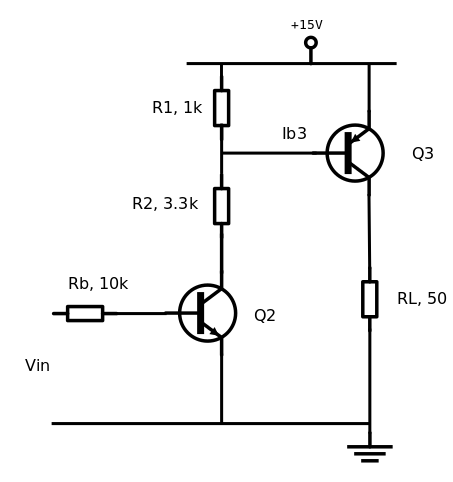
\includegraphics[scale=0.5]{images/switch_2_bjt.png}
\end{figure}

\subsection{Analysis}

\paragraph{Q2 closed - $V_\text{in} = 0V$}: Q2 is open and its collector at a voltage of 15V. The base of Q3 is also at 15V and therefore Q3 is off. Its emitter is at zero voltage and the current through $R_L$ is zero.

\paragraph{Q2 opened - $V_\text{in} = 3V$}: Q2 opens, the voltage at its collector is $\approx 0V$. The collector current of Q2 is therefore

\bee
\frac{(15-0.6)V}{3.3k\Omega} \approx 4.4mA
\eee
%
Therefore the base current of Q2 is estimated with $4.4mA / 25 \approx 180\mu A$ (with an estimated current gain of 25). This requires a base resistor $R_b$ of about $3V/180\mu A \approx 17k\Omega$. We took $10k\Omega$ to ensure Q2 is deeply saturated.

The $4.4mA$ from above are driven by two sources: (i) Via $R_1$, but note that this current is only about $0.6V / 1k\Omega \approx 0.6mA$ (because Q3 is open, its base is $\approx 0.6V$ \emph{lower} than its emitter - this is a PNP transistor!), and (ii) from the base of Q3 which therefore must be $4.4mA - 0.6mA \approx 3.8mA$.
%
Since Q3 is open, its emitter of Q3 is at $\approx 15V$ as Q3 is open and the current through $R_L$ is about $15V / 50\Omega \approx 300mA$.


\subsection{Simulation}

The following ngspice netlist describes the circuit from above.

\begin{verbatim}

.model mnpn npn is=1e-16
.model mpnp pnp is=1e-16

vcc vplus gnd dc 15V
vin in gnd dc 3V

*   C   B   E
q2 q2c q2b gnd    mnpn
q3 rl  q3b vplus  mpnp

Rb in q2b 10kOhm

R1 vplus q3b    1kOhm
R2 q3b q2c 3.3kOhm

Rload gnd rl 50Ohm

.end
\end{verbatim}

It can be loaded into ngspice by (i) starting ngspice with the netlist filename as parameter, or (ii) inside ngspice with \verb! source <filename>!.

Simulating the operating point can be triggered with \verb op (and changing the vin voltage). Voltages can then be printed via \verb! print v(<node>)!; e.g. \verb! print v(q3b)! yields $14.1V$. A \verb show shows information about the bipolar transistors; we see that the B-E voltage of Q3 is $\approx 0.9V$ (and not $0.6V$ as used above).

However, simulation does not provide information about other currents; e.g. through resistors. We therefore need to add voltage sources (with zero voltage) in series whereever we want to measure a current.

The netlist therefore looks as follows (with vr1, vr2, and vrload being such dummy voltage sources).

\begin{verbatim}

.model mnpn npn is=1e-16
.model mpnp pnp is=1e-16

vcc vplus gnd dc 15V
vin in gnd dc 3V

*   C   B   E
q2 q2c q2b gnd    mnpn
q3 rl  q3b vplus  mpnp

Rb in q2b 10kOhm

R1 vplus r1temp    1kOhm
R2 q3b r2temp 3.3kOhm

vr1 r1temp q3b dc 0V
vr2 r2temp q2c dc 0V
vrload rl rltemp dc 0V

Rload gnd rltemp 50Ohm

.end

\end{verbatim}

Issuing \verb!show! now displays the required currents. It shows - e.g. - that the current through $R_2$ is $\approx 4.24mA$.


\paragraph{DC Sweep.} Finally, we want to sweep the input voltage and display the emitter voltage of Q3 as function of the input voltage. To this end, we include the line \verb!.dc vin 0 2 0.01! towards the end of the netlist file. After (re)loading, we can run the simulation with \verb!run!. Either we plot the thing directly in ngspice \verb!plot v(rl)! or we export the data as table \verb!wrdata rl_voltage rl! and plot it via Julia.

The following plot shows the result: The threshold is at $\approx 1V$ and quite steep (from $0.8V$ to $1.2V$).

\begin{figure}[htb]
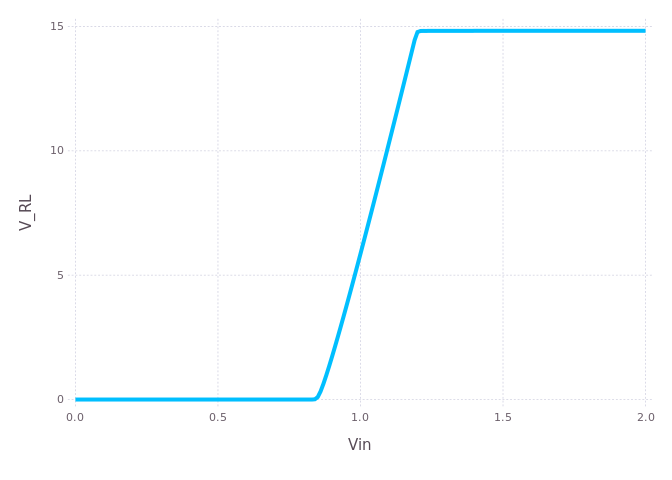
\includegraphics[scale=0.5]{images/rl_voltage.png}
\end{figure}






\DiaryEntry{Linear Block Codes}{2017-03-27}{Coding}


\subsection{Definition}

An $(n,k)$ binary block code $\Cc$ is a set of $2^k$ n-vectors called code words. An enocder maps a messsage $m$ (a length-k binary word) to the associated code word $c$.

A \emph{linear} code is a code where the $k$ code words form a $k$-dimensional vector subspace of the vector space of all length-$n$ binary words. In other words, the linear combination of two (or more) codewords is again a codeword.

$n$ is said to be the length of the Code and $R=k/n$ is the code rate.

The Hamming weight $wt(c)$ of a codeword is the number of ones of a codeword $c$. The minimum weight of a code $\Cc$ is the smallest Hamming weight of any non-zero codeword. For a linear code, the minimum distance equals the minimum weight.


\subsection{Generator Matrix Description}

Since a linear block code is a $k$-dimensional vector space, there exists a base of $k$ independent vectors $g_0, g_1,\ldots,g_{k-1}$ for this vector space. Every codeword $c$ can then be represented as linear combination according to

\bee
c = m_0 g_0 + \cdots + m_{k-1} g_{k-1}
\eee
%
In coding, we represent vectors as row vectors; collecting the set of basis vectors in a matrix yields the matrix $G$

\bee
G = \begin{bmatrix} g_0 \\ g_1 \\ \cdots \\ g_{k-1} \end{bmatrix}
\eee
%
Collecting the message into a length-$k$ vector $m = [m_0 \cdots m_{k-1}]$ we can write the encoding operations as

\bee
c = m G
\eee
%
In case of a systematic code, the message bits $m_0 ... m_{k-1}$ can be found unchanged in the encoded message $c$; typically, the last $k-1$ elements of $c$ contain the message bits. Note that a code need not be linear; being systematic is a general characterisitc of any code.

For such a systematic linear block code, we can write the matrix $G$ as $G=[P I_k]$, with the matrix $P$ generating the parity check bits and the $k\times k$ identity matrix. The encoding oeration then becomes

\bee
c = mG = m [P I_k] = [mP m]
\eee
%
which shows that the message bits are located at the end of the codeword. 


\subsection{Parity Check Matrix}

The dual code $\Cc^\star$ of a code $\Cc$ is an $(n, n-k)$ code. The $n-k+1$-dimensional basis for the corresponding vector space is the set of vectors $h_0, h_1, \ldots, h_{n-k+1}$ which we again collect in a matrix $H$

\bee
H = \begin{bmatrix} h_0 \\ h_1 \\ \cdots \\ h_{n-k+1} \end{bmatrix}
\eee
%
which is called the parity check matrix. The generator matrix $G$ and the parity check matrix $H$ are connected via

\bee
GH^T = 0
\eee
%
A vector $v$ is a codeword of a code $\Cc$, iff

\bee
vH^T = 0
\eee
%
In case of a systematic linear code, the parity check matrix is given by

\bee
H = [I_{n-k} -P^T] = [I_{n-k} P^T]
\eee


\subsection{Decoding}

\subsubsection{Syndrome}

The syndrome $s$ is calculated via $s = rH^T$ and we have $s=0$ iff $c \in \Cc$.

Assume we transmit the codeword $c = mG$ across a faulty channel which introduces random faults $e$ and receive

\bee
r = c + e
\eee
%
Then the syndrome becomes

\bee
s = (c+e)H^T = cH^T + eH^T = eH^T
\eee


\subsubsection{The Standard Array}

For maximum likelihood decoding, we need to perform the following operation

\bee
\hat{c} = \arg \min_{c \in \Cc} d_H(c,r)
\eee
%
i.e. we choose the codeword being closest (in terms of Hamming distance) to the received word $r$.
%
Let the set of codewords be $\{c_0, c_1,\ldots\}$ and let $V_i$ denote the set of codewords closer to $c_i$ than any other codeword. Vectors having the same distance to more than one codeword are assigned at random to any $V_i$. The sets $V-i$ partition the space of length-n words into $2^k$ disjoint subsets. ML decoding can be alternatively interpreted as determining the set $V_i$ a received word falls into.

The standard array is a representation of this partitioning. It is a table, with the $2^k$ codewords on top. The words of the set $V-i$ are then contained in the $i$-th column. The standard array can be obtained as follows:

\begin{itemize}

\item Write down all codewords as the first row of the array.

\item From the remaining \emph{unused} words, select one with minimum weight and write it into the first column (the column with the all-zero codeword on top). Add the word to the codewords of all other columns.

\item Repeat word selection and proceed as above until all words have been used. 

\end{itemize}


\subsection{Example}

Consider the generator matrix for a $(7,3)$ code

\bee
G = \begin{bmatrix} 0 &1 &1 &1 &1 &0 &0\\
                    1 &0 &1 &1 &0 &1 &0 \\
                    1 &1 &0 &1 &0 &0 &1 \end{bmatrix}
\eee

As outlined above, we will first obtain the codewords by iterating over all $2^3$ message words. Message $[0 0 0]$ yields $[0 0 0 0 0 0 0]$, message $[0 0 1]$ yields $[1 1 0 1 0 0 1]$ and so on.

Let's write the message words and the corresponding codewords into a table like this (we take the MSB to be on the righmost position!!)

\bee
\begin {array}{ccccccccc}
& 000     & 100     & 010     & 110     & 001     & 101     & 011     & 111 \\
& 0000000 & 0111100 & 1011010 & 1100110 & 1101001 & 1010101 & 0110011 & 0001111
\end{array}
\eee

An unused codeword of weight 1 is $[10000000]$; when we add it to the second row (which contains the codewords), we obtain

\bee
\begin{array}{ccccccccc}
         & 000     & 100     & 010     & 110     & 001     & 101     & 011     & 111 \\
         & 0000000 & 0111100 & 1011010 & 1100110 & 1101001 & 1010101 & 0110011 & 0001111 \\
10000000 & 1000000 & 1111100 & 0011010 & 0100110 & 0101001 & 0010101 & 1110011 & 1001111
\end{array}
\eee

We can continue like this and obtain a table like the following. 

\begin{figure}[htb]
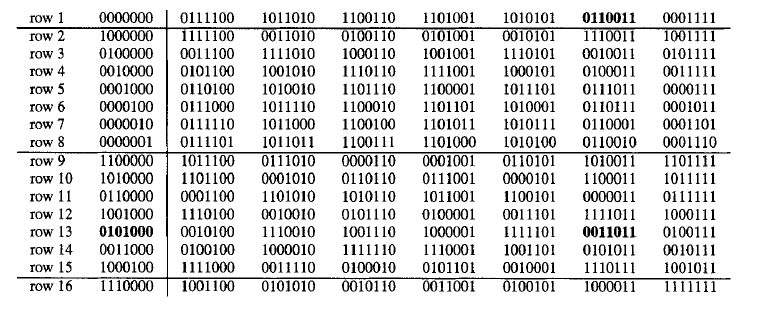
\includegraphics[scale=0.8]{images/standard_array.png}
\end{figure}

From the table we make the following observations:

\begin{itemize}

\item The difference or sum of two words in the same row is a codeword because $(c_i + e_k) \pm (c_j + e_k) = c_i + c_j$ and the sum / difference of two codewords is again a codeword.

\item The words in the same row are all different; If we had $c_i + e = c_j + e$, $c_i = c_j$ would follow which is impossible.

\item The rows of the standard array are cosets as each row is of the form $e + \Cc = \{e + c: c \in \Cc\}$ and the elements in the first column are called coset leaders.

\item The minimum weight of the codewords is $4$ bits.

\item All $1$-bit errors can be corected, $7$ $2$-bit errors can be corrected, and one $3$-bit error can be corrected.

\end{itemize}


\subsection{Syndrome Decoding}

Decoding by means of the standard array is complicated as the table soon becomes infeasibly big. Syndrome decoding is simpler.

It is based on the observation that - for a given error word $e$ - the syndrome does \emph{not} depend on the sent codeword; i.e.

\bee
s = rH^T = eH^T
\eee
%
Syndrome decoding works with a precalculated mapping between syndrome and error word. For every possible syndrome, the error word is calculated. In case several error patterns lead to the same syndrome (this is possible as there are $2^n$ error patterns and only $2^k$ syndromes), the minimum weight error word is taken. 

When a (possibly wrong) codeword is received, the decoder calculates the syndrome. If it is zero, the decoder passes on the received codeword; otherwiese, the decoder looks up the corresponding error pattern, adds the pattern to the received codeword and passes on the result. In any case, a subsequent stage extracts the message bits from the codeword (simple in case of a systematic code).

Continuing the example above, consider the syndrome $[1 1 0 1]$. It is caused by the follwing error patterns: $[0,1,1,0,0,1,0]$, $[1,1,0,0,1,1,1]$, $[1,1,0,1,0,0,0]$, $[1,0,1,1,0,1,1]$, $[0,1,1,1,1,0,1]$, $[0,0,0,0,0,0,1]$, $[0,0,0,1,1,1,0]$, $[1,0,1,0,1,0,0]$. By the description above, the associated error pattern in the syndrome decoding table will be $[0,0,0,0,0,0,1]$; i.e. the error pattern with lowest weight.




\DiaryEntry{Graphs, General}{2017-04-04}{Graphs}

\subsection{Global Graph Properties}

As a first graph theorem, we consider

\begin{theorem}
  A finite graph has an even number of vertices with odd degree.
\end{theorem}



As an example consider the following graph (actually, the whole blog entry is an execuse to play around with tikz ;-) ).

\begin{figure}[H]
\centering
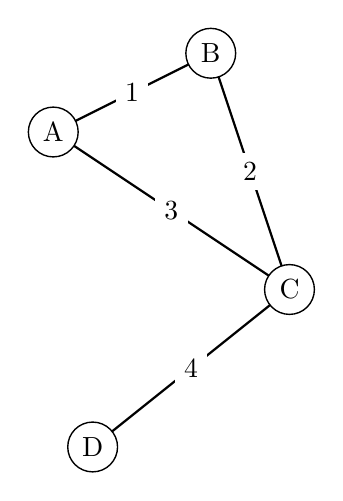
\begin{tikzpicture}[transform shape]
  \Vertex[x=0,y=0]{A}
  \Vertex[x=2,y=1]{B}
  \Vertex[x=3,y=-2]{C}
  \Vertex[x=0.5,y=-4]{D}
  \Edge[label=1](A)(B)
  \Edge[label=2](B)(C)
  \Edge[label=3](A)(C)
  \Edge[label=4](D)(C)
\end{tikzpicture}
\caption{Example Graph, I.}
\end{figure}

which we can represent via a table listing edges and vertices as follows:

\bee
\begin{array}{c|c}
edge & vertices\\
\hline
1 & A,B\\
2 & B,C\\
3 & A,C\\
4 & C,D
\end{array} 
\eee
%
The idea for the proof is to count the number of vertices in the right column in two different ways:

\begin{itemize}
\item The number of entries in the right column is two times the number od edges. In the example graph, we have $4$ edges, and $2\times 4 = 8$ entries in the right column.

\item The degree of a vertex is equal the number of times it occurs in the table. In the example graph, e.g. the vertex A has degree and occurs two times in the table. Summing over the degree of all vertices yields the number of entries in the right column.

\end{itemize}

Equating both sides therefore yields

\bee
\sum_{x \in \Vc(G)} \deg(x) = 2 |\Ec(G)|
\eee
%
A bit less formal proof, is the observation that summing over all edge degrees counts the edges twice; in the example graph, edge 1 is counted when we add the degree of vertex ``A'' and the degree of vertex ``B''. This also yields above equation.
%
Anyway, looking at the equation, we observe the following

\begin{itemize}

\item The righ-hand side is even.

\item For the left-hand side, we see that a sum with an even number of odd terms is even (e.g. $1 + 1 = 2$, $1+3+3+1 = 8$).
  
\end{itemize}

This proves the theorem stated above. \qed

In the example graph above, verices ``C'' and ``D'' had odd degree; wWe can play around a bit further and add another vertex to the graph like below.

\begin{figure}[H]
\centering
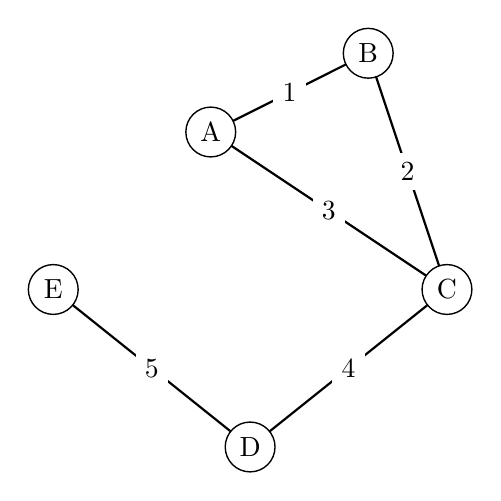
\begin{tikzpicture}[transform shape]
  \Vertex[x=0,y=0]{A}
  \Vertex[x=2,y=1]{B}
  \Vertex[x=3,y=-2]{C}
  \Vertex[x=0.5,y=-4]{D}
  \Vertex[x=-2,y=-2]{E}
  \Edge[label=1](A)(B)
  \Edge[label=2](B)(C)
  \Edge[label=3](A)(C)
  \Edge[label=4](D)(C)
  \Edge[label=5](D)(E)
\end{tikzpicture}
\caption{Example Graph, II.}
\end{figure}

Vertex ``C'' has still odd degree, but vertex ``D'' now has even degree and the new vertex``E'' has odd degree: The number of vertices with odd degree is still even.


\subsubsection{Complete Graphs}

In a complete graph with $n$ vertices, all vertices are connected with each other. To calculate the number of edges, we observe that every vertex is connected with the remaining $n-1$ vertices. If we take $n(n-1)$, we count every edge double; Therefore, the total number of edges is

\bee
|\Ec(\Gc)| = \frac{n(n-1)}{2}
\eee

Some examples of complete graphs are shown below. For $n=3$ vertices we have $\frac{3 \times 2}{2} = 3$ edges, for $n=4$ vertices we have $\frac{4 \times 3}{2} = 6$ edges, and for $n=5$ vertices we finally have $\frac{5 \times 4}{2} = 10$ edges.

\begin{figure}[H]

\begin{subfigure}{0.4\textwidth}
  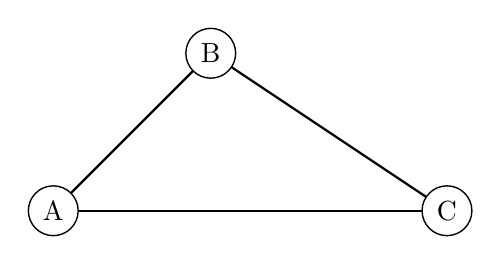
\begin{tikzpicture}[scale=1.0, transform shape]
    \Vertex[x=0,y=0]{A}
    \Vertex[x=2,y=2]{B}
    \Vertex[x=5,y=0]{C}
    \Edge(A)(B)
    \Edge(B)(C)
    \Edge(A)(C)
  \end{tikzpicture}
\caption{$n=3$ vertices.}
\end{subfigure}
\qquad % this is important, otherwise the figures won't be next each other...
\begin{subfigure}{0.4\textwidth}
  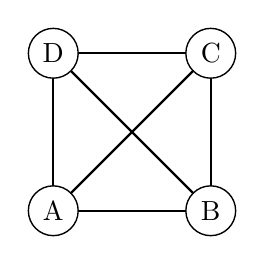
\begin{tikzpicture}[scale=1.0, transform shape]
    \Vertex[x=0,y=0]{A}
    \Vertex[x=2,y=0]{B}
    \Vertex[x=2,y=2]{C}
    \Vertex[x=0,y=2]{D}
    \Edge(A)(B)
    \Edge(A)(C)
    \Edge(A)(D)
    \Edge(B)(C)
    \Edge(B)(D)
    \Edge(C)(D)
  \end{tikzpicture}
\caption{$n=4$ vertices.}
\end{subfigure}
\end{figure}



\begin{problem}
We have a disconnected graph with $10$ vertices. Show that this graph has at most $36$ edges.
\end{problem}

Since the graph is disconnected, it contains of (at least) two components. Assume the first component has $m$ vertices, the other $10 - m$. The total number of edges is then

\bee
|\Ec(\Gc)| = \frac{m(m-1)}{2} + \frac{(10-m)(10-m-1)}{2}
\eee

We guess that this expression attains its maximum of $36$ at $m=1$ and $m=9$. In these extreme cases (one component with $9$ vertices, the other component with just $1$ vertex), the total number of edges is $36$; in all other cases it is less and this completes the proof. \qed 



\subsection{Eulerian Graph}

\begin{definition}
A closed path through a graph which uses every edge exactely once is called an Eulerian circuit. A finite graph with no isolated vertices that contains such a path is an Eulerian graph.
\end{definition}

There is a condition on whether a graph is Eulerian or not stated in the following theorem.

\begin{theorem}
A finite graph with no isolated vertices is Eulerian iff it is connected and every vertex has evn degree.
\end{theorem}

The path enters a vertex through some edge and leaves by another edge; therefore all verices must have even degree. To show that this condition is sufficient, start in a vertex ``A'' and begin a path. Keep going, not using the same edge twice until we cannot go further. Since every vertex has even degree, this can only happen when we return to ``A'' and we have used all edges from ``A''. If there are unsued edges from ``A'', we start making another path from / to these edges until all edges are used up. Finally, shorter paths can be combined into longer ones until the complete graph has been traversed. \qed

\paragraph{Example.} Some simple examples are shown in the following Figure. On the left, the simplest Eulerian circuit construction starts in vertex ``A'' and goes along ``B'', ``C'', ``D'', ``E'', returns to ``A'' from there. Slightly trickier is to start in ``B'', go via ``C'', ``D'' back to ``B''. However, not all edges from ``B'' are used, so we start another walk from ``B'' via ``A'', ``E'' and back to ``B''. The Eulerian circuit is then the combination of these two paths. On the right, we can also start in ``B'' and create two subpaths as above: ``B'', ``C'', ``D'', ``B'' and ``B'', ``E'', ``A'', ``B''. This leaves the path ``E'', ``F'', ``D'', ``G'', ``E'' out. However, we merge these three paths into one Eulerian circuit.

In any case, note that all paths have vertices with even degree.

\begin{figure}[H]

\begin{subfigure}{0.4\textwidth}
  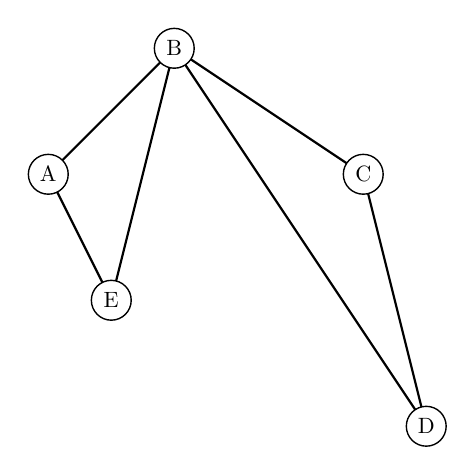
\begin{tikzpicture}[scale=0.8, transform shape]
    \Vertex[x=0,y=0]{A}
    \Vertex[x=2,y=2]{B}
    \Vertex[x=5,y=0]{C}
    \Vertex[x=6,y=-4]{D}
    \Vertex[x=1,y=-2]{E}
    \Edge(A)(B)
    \Edge(B)(C)
    \Edge(C)(D)
    \Edge(B)(D)
    \Edge(A)(E)
    \Edge(B)(E)
  \end{tikzpicture}
\caption{Euler, I.}
\end{subfigure}
\qquad % this is important, otherwise the figures won't be next each other...
\begin{subfigure}{0.4\textwidth}
  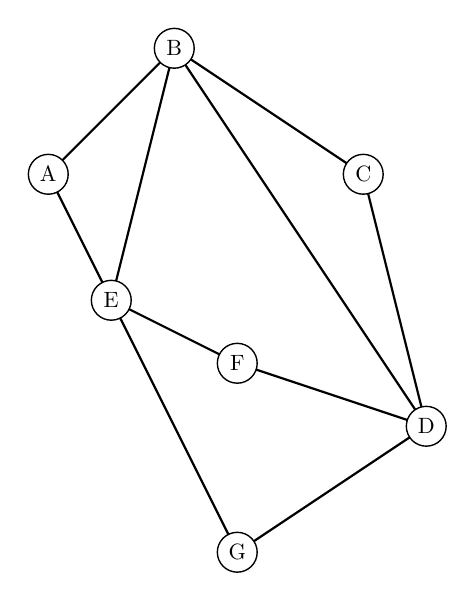
\begin{tikzpicture}[scale=0.8, transform shape]
    \Vertex[x=0,y=0]{A}
    \Vertex[x=2,y=2]{B}
    \Vertex[x=5,y=0]{C}
    \Vertex[x=6,y=-4]{D}
    \Vertex[x=1,y=-2]{E}
    \Vertex[x=3,y=-3]{F}
    \Vertex[x=3,y=-6]{G}
    \Edge(A)(B)
    \Edge(B)(C)
    \Edge(C)(D)
    \Edge(B)(D)
    \Edge(A)(E)
    \Edge(B)(E)
    \Edge(E)(F)
    \Edge(E)(G)
    \Edge(D)(F)
    \Edge(D)(G)
  \end{tikzpicture}
\caption{Euler, II.}
\end{subfigure}
\end{figure}

\DiaryEntry{Graphs, Trees}{2017-04-11}{Graphs}

\subsection{General}


\begin{definition}
A graph is called a tree if it is connected and contains no cycle as a subgraph.
\end{definition}

The two defining properties are somewhat opposite: The connectedness part ensures that the graph does not have ``too few'' edges, whereas the ``no cycles'' part ensures that the graph has not ``too many'' edges.

If a graph is connected, then it will stay connected when we add another edge. If we remove an edge, the graph may become disconnected. If a graph has no cycles, it will still have no cycles if we remove another edge. If a graph has no cycles, it may become cycles if we add another edge.

In that sense a tree is a ``minimally connected'' subgraph or a ``maximally cycle-free'' graph:

\begin{theorem}
(i) A graph is a tree if and only if it is connected, but deleting any of its edges results in a disconnected graph. (ii) A graph is a tree if and only if it contains no cycles, but adding any new edge creates a cycle.
\end{theorem}

For (i) we want to show that a tree cannot stay connected if we remove an edge. Assume that the edge $u-v$ is deleted from the graph $G$ and the resulting graph $G'$ stays connected. This implies that there is a path from $u$ to $v$. However, if we put the edge $u-v$ back, the path and the edge $u-v$ will form a cycle and that contradicts the definition of a tree.

(ii) follows with a similar argument.

Assume we have a connected graph with $n$ nodes and an edge $e$. If we obtain a disconnected graph by deleting $e$, then $e$ is called a cut-edge. With this definition, every edge of a tree is a cut-edge.

A spanning tree of a graph is a subgraph that has the same nodes but is a tree. We can obtain a spanning tree from a graph by deleting edges from the graph until a graph is obtained that is still connected, but deleting any further edge makes it disconnected; by definition, this is a tree. The edge deletion process can be carried out in many different ways; therefore, the spanning tree of a graph is not unique.

\begin{theorem}
  Every tree on $n$ vertices has $n-1$ edges.
\end{theorem}

We can prove this via induction: We start the tree with two vertices and an edge connecting the two. Adding one edge after the other, keeps the different between the number of edges and the number of vertices the same.

The converse, however is not true; i.e. a graph with $n$ vertices and $n-1$ edges is not necessarily a tree. Consider the example below.

\begin{figure}[H]
\centering
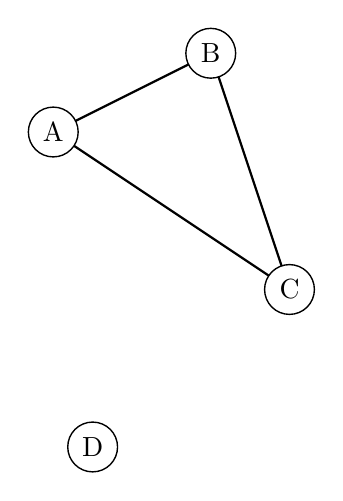
\begin{tikzpicture}[transform shape]
  \Vertex[x=0,y=0]{A}
  \Vertex[x=2,y=1]{B}
  \Vertex[x=3,y=-2]{C}
  \Vertex[x=0.5,y=-4]{D}
  \Edge(A)(B)
  \Edge(B)(C)
  \Edge(A)(C)
\end{tikzpicture}
\caption{Trees.}
\end{figure}




\DiaryEntry{Cyclic Codes, I}{2017-04-18}{Coding}

\subsection{Repetition - Rings}

\begin{definition}
  A ring $(R,+,\cdot)$ is a set $R$ with two binary opeations, $+$ (addition) and $\cdot$ (multiplication), defined on $R$ such that

  \begin{itemize}
    \item $(R,+)$ forms an abelian group with additive identity typically denoted as $0$.
    \item The multiplication operation $\cdot$ is associative: $(a \cdot b) \cdot c = a \cdot (b \cdot c)$ for $a,b,c \in R$.
    \item Left and right distributive laws hold: $a(b+c) = ab + ac, (a+b)c = ac + bc$
  \end{itemize}
%
  A ring is commutative if $a \cdot b = b \cdot a$, for all $a,b \in R$. A ring is said to be a ring with identity if $\cdot$ has an identitiy element which is typically denoted as $1$.

\end{definition}

As a simple example, consider $(\mZ_6, +, \cdot)$ with addition and multiplication tables as follows (addition and multiplication are taken modulo-6):

\begin{figure}[H]
  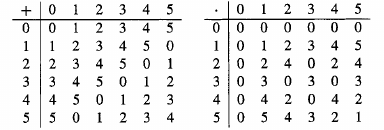
\includegraphics[scale=0.75]{images/cyclic_codes_01.png}
\end{figure}

Note that the set does not form a group under multiplication (it does under addition, though). However, this does not contradict the ring definition; i.e. it is a ring.


\subsection{Repetition - Rings of Polynomials}

If $R$ is a ring, then the set of all polynomials with coefficients in $R$ form a ring under the usual operations for polynomial addition and multiplication. This ring is denoted as $R[x]$, where $x$ is the polynomial variable:

\bee
f(x) = \sum_{i=0}^n a_i x^i, a_i \in R
\eee

Addition (adding coefficients with the same degree according to the ring operation) of polynomials yields another polynomial in the ring, the same holds for multiplication. The inverrse of a polynomial will in general not be another polynomial (e.g. $(1 + 4x)^{-1}$), but note that a ring need not have multiplicative inverses (it's not a field after all).

\paragraph{Example.} Taking $R$ to be $(\mZ_6, +, \cdot)$, we obtain a polynomial ring as $R[x]$ with some example elements $f_1(x) = 3 + x, f_2(x) = 5 + 3x^2$. For example, we have $f_1 + f_2 = 2 + x + 3x^2$ and $f_1 f_2 = 3 + 5x + 3x^2 + 3x^3$.

\subsection{Repetition - Quotient Rings}

In Group Theory, a set of cosets was created by ``translating'' a subgroup; i.e. if $H$ is a subgroup of a group $G$, then we formed cosets by $g + H, g \in G$.

In a similar spirit, we can collect polynomials over a ring into equivalence classes by their remainder after division by a fixed polynomial.

As an example, consider the ring of polynomials $GF(2)[x]$ and a fixed polynomial $x^3+1$. Now collect all polynomials with remainder $0$ after division modulo $x^3+1$:

\bee
S_0 = \{0, x^3+1, x^4+x, x^5+x^2, \ldots\} = \langle x^3 + 1 \rangle
\eee

where $S_0 = \langle x^3 + 1 \rangle$ is the set of polynomials generated by $x^3+1$. Note that $S_0$ is actually a subring: Denote $p_1(x), p_2(x)$ two polynomials with remainder $0$ after division by $x^3+1$. The sum $p_1(x) + p_2(x)$ will also have a remainder $0$ after division by $x^3+1$

\bee
\frac{p_1(x) + p_2(x)}{x^3+1} = \frac{p_1(x)}{x^3+1} + \frac{p_2(x)}{x^3+1} \equiv 0 \bmod (x^3+1)
\eee

and in a similar spirit, the multiplication as well

\bee
\frac{p_1(x)p_2(x)}{x^3+1} = \frac{p_1(x)}{x^3+1} \frac{p_2(x)}{x^3+1} \equiv 0 \bmod (x^3+1)
\eee

The set $S_1$ contains all polynomials with remainder $1$ after division modulo $x^3+1$:

\bee
S_1 = \{1, x^3, x^4+x+1, x^5+x^2+1, \ldots\} = 1 + \langle x^3 + 1 \rangle
\eee

Noe that his is not a (sub)ring as it does not contain the identity element. The other equivalence classes are obtained in the same manner.

\begin{figure}[H]
  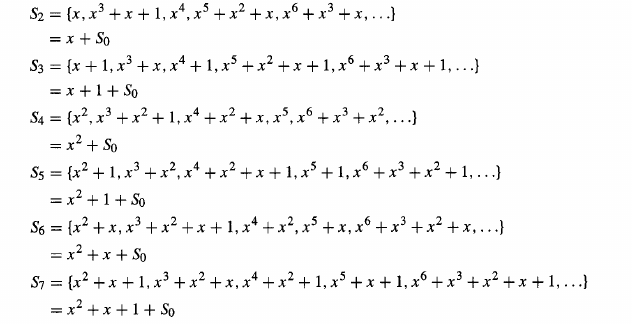
\includegraphics[scale=0.65]{images/cyclic_codes_02.png}
\end{figure}

By dividing through $x^3+1$, only 7 different remainders are possible: $0, 1, x, 1+x, 1+x^2, x+x^2, 1+x+x^2$. Therefore, all polynomials of $GF(2)[x]$ fall into of these equivalence classes.

In a similar spirit to defining an induced operation of cosets, we can define induced operations $+$ and $\cdot$ for the equivalence classes of polynomials modulo $x^3+1$ by operation on representative elements. We obtain the following tables:

\begin{figure}[H]
  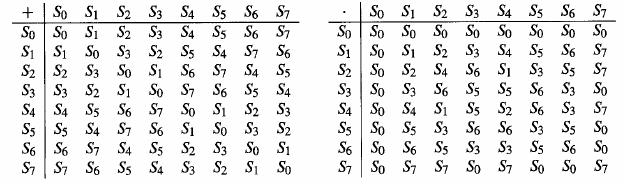
\includegraphics[scale=0.65]{images/cyclic_codes_03.png}
\end{figure}

As an example, note that $S_3 + S_5 = S_6$. Adding one of the corresponding elements from the cosets yields $(x+1) + (x^2+1) \equiv x^2+x$, which corresponds to $S_6$. For multiplication, let us take $S_3 S_7 = S_0$, corresponding to the following polynomial identitiy: $(x+1)(x^2+x+1) \equiv x^3+1$ which corresponds to $S_0$.

If we define $R=\{S_0, S_1,\ldots, S_7\}$, then $(R,+)$ is an Abelian group with $S_0$ as identity and for multiplication $S_1$ acts as identity. Not every element has a multiplicative inverse, so $R - S_0$ is not a group. However, the whole thing $(R,+,\cdot)$ is a ring denoted as $GF[x]/\langle x^3+1 \rangle$.

In the general case, denote a ring $GF(2)[x]/\langle x^n-1 \rangle$ as $R_n$ and a ring $\mF_q[x]/\langle x^n-1\rangle$ as $R_{n,q}$.

\paragraph{General Case.} For a field $\mF$ (with $q$ elements), the associated ring of polynomials $\mF[x]$ can be partitioned by a polynomial $f(x)$ of degree $m$ into $q^m$ different equivalence classes with one equivalence class for each remainder modulo $f(x)$. This ring is denoted as $\mF[x]/\langle f(x)\rangle$ or $\mF[x]/f(x)$.

As a side note (which will be proven later on), we note that the ring $\mF[x]/f(x)$ is a field iff the polynomial $f(x)$ cannot be factored over $\mF[x]$. In the example above, we have $x^3+1 = (x+1)(x^2+x+1)$ so $\mF[x]/(x^3+1)$ is not a field.



\subsection{Ideals in Rings}

\begin{definition}
  Let $R$ be a ring. A nonempty subset $I \subseteq R$ is an ideal if

  \begin{itemize}
    \item $I$ forms a group under addition in $R$.
    \item For any $a \in I$ and $r \in R$, $ar \in I$.
  \end{itemize}
\end{definition}

The first point ensures that the ideal has a structure; i.e. adding two ideal elements yields another ideal element. The second point is interesting in that the product of an ideal and a ``non-ideal'' element is still an ideal.

As a simple example, take $R$ as the set of integers. An ideal is the set of even numbers; the sum of any two even numbers is even and the product of any number with an even one gives an even number.

\begin{definition}
  An ideal $I$ in a ring $R$ is said to be principal if there exists some $g \in I$ such that every element $a \in I$ can be expressed as a product $a = mg$ for some $m \in R$. For a principal ideal, such an element $g$ is called the generator element. The ideal generated by $g$ is denoted as $\langle g \rangle$:

  \bee
    \langle g \rangle = \{hg : h \in R\}
  \eee
  
\end{definition}

The ideal in the example above is principal with a generator element $g = 2$. Every element of the ideal can be created by $2m$ with $m \in R$.

\begin{theorem}
  Let $I$ be an ideal in $\mF_q[x] / \langle x^n-1 \rangle$. Then
  \begin{itemize}
    \item There is a unique monic polynomial $g(x) \in I$ of minimal degree.
    \item $I$ is principal with generator $g(x)$.
    \item $g(x)$ divides $(x^n-1)$ in $\mF_q[x]$.
  \end{itemize}

\end{theorem}

\paragraph{Example.}Consider the polynomial $x^7+1$ over $GF(2)[x]$ which can be factored as

\bee
x^7 + 1 = (x+1)(x^3 + x + 1)(x^3 + x^2 + 1)
\eee

This factorization can be obtained in GAP via the following commands

\begin{verbatim}
a:=GF(2);
x:=X(GF(2));
Factors(p);
   [ x_1+Z(2)^0, x_1^3+x_1+Z(2)^0, x_1^3+x_1^2+Z(2)^0 ]
\end{verbatim}

Any combination of these 3 factors can be used as generator for a principal ideal.

\paragraph{Example.} A simpler example uses the polynomial $p(x) = x^3+1 = (x+1)(x^2+x+1)$. Choosing as generator $g_1(x) = x+1$, we can calculate the ideal by multiplying $g_1(x)$ with the elements of $GF(2)[x]/x^3+1 = \{0,1,x,1+x, x^2, x^2+1, x^2+x, x^2+x+1\}$ (and taking modulo-$x^3+1$). We can do this in GAP with the following script

\begin{verbatim}
a:=GF(2);
x:=X(GF(2));

# let's take the first factor, x+1 as generator for an ideal

GElements := [0,1,x,1+x,x^2,x^2+1,x^2+x, x^2+x+1];
p1 := x+1;

for e in GElements do
   Print(e,"...", e*p1 mod p, "\n");
od;
\end{verbatim}

There are some duplicates; after removal of them we obtain the ideal $I_1 = \{0, x+1, x^2+1, x^2+x\}$. The sum of two ideal elements is again an ideal element (``proof'' by going over all combinations) and the product of an ideal element and any element of $GF(2)[x]/x^3+1$ is again in the ideal $I_1$ (``proof'' by going over all combinations).

\subsection{Cyclic Codes}

A cyclic shift of a binary code word looks like this: We have a vector $\cbf = (c_0, c_1, \ldots,c_{n-2}, c_{n-1})$ and shift it cyclically to the right to obtain $\cbf' = (c_{n-1}, c_0, c_1, \ldots, c_{n-2})$.

\begin{definition}
  An $(n,k)$ block code is cyclic, it it is linear and if for every codeword, its right cyclic shift is also a codeword.
\end{definition}


This cyclic shifting can be expressed in terms of polynomial manipulations; If we have the codeword

\bee
\cbf = (c_0, c_1, \ldots,c_{n-2}, c_{n-1})
\eee
%
we can associate the polynomial

\bee
c(x) = \cbf = c_0 + c_1 x + c_2 x^2 + \cdots c_{n-1} x^{n-1}
\eee
%
A non-cyclic right-shift is then represented as $xc(x)$ and a cyclic right-shift is represented by $xc(x) \mod (c^n-1)$.


\end{document}
